% AMS Weather and Forecasting manuscript (submission / peer-review format)
% Class: official AMS LaTeX Template v6.1 (draft mode: 12 pt, ~1.5 line spacing,
% 1-inch-class margins, line numbers). Do not use the [twocol] option for submission.
%
% Compile twice: pdflatex waf_manuscript.tex
%
% Figure files sit in this folder (no directory paths in \includegraphics).
\documentclass{ametsocv6.1}

% Packages already loaded by ametsocv6.1.cls: graphicx, amsmath, natbib, url,
% setspace, lineno, xcolor, newtxtext/newtxmath. Do not reload them.
\usepackage{booktabs}
\usepackage{multirow}
\usepackage{placeins}

\newcommand{\sece}{SECE}
\newcommand{\bob}{Bay of Bengal}
\newcommand{\era}{ERA5}
\newcommand{\ibtracs}{IBTrACS}

\title{ERA5-Augmented Ensemble Learning for Multi-Horizon Tropical Cyclone
Track Prediction over the Bay of Bengal: A Leakage-Aware Benchmark}

\authors{
Author One,\aff{a}\correspondingauthor{Author One, [email]}
and Author Two\aff{a}
}

\affiliation{
\aff{a} [Department, Institution, City, Country]
}

\abstract{
Accurate short- to medium-range cyclone track forecasting is a foundational input
to early warning over the Bay of Bengal, a basin that combines complex monsoon-season
steering with some of the highest coastal population exposure in the world. We
present a rigorously validated benchmark of eight track-prediction systems, a
proposed Subset-Expert Context-Aware Ensemble (SECE v2 Phase~3) and seven
baselines spanning tree and hybrid families, evaluated at 3, 12, 24, and 48\,h
lead times on North Indian Ocean IBTrACS storms with genesis in 1940--2024.
After quality control the modelling table contains 852 storms and 27{,}728
three-hourly forecast origins, of which 583 storms and 15{,}605 origins support
multi-horizon supervision. Forty-nine kinematic and derived predictors are
augmented with 14 ERA5 reanalysis fields collocated at the storm centre,
comprising winds at 850, 500, and 200\,hPa, mean sea level pressure, sea surface
temperature, a derived deep-layer steering wind, and vertical wind shear.
Critically, we identify and correct a subtle form of test-set leakage present in
an earlier iteration of our own development, in which architectural decisions
were guided by repeated inspection of test-set performance; we replace it with a
two-tier protocol in which nine development seeds carry all design decisions and
nine disjoint held-out seeds are evaluated exactly once. On the held-out confirm,
pooled over 442 distinct test storms, SECE attains median great-circle errors
of 4.895, 35.538, 101.186, and 246.331\,km. Paired Wilcoxon signed-rank tests
with Bonferroni correction across seven comparisons show that SECE is
significantly better than every baseline at 3 and 12\,h ($p<0.0071$),
statistically indistinguishable from the strongest stacks at 24 and 48\,h, and
never significantly worse than any baseline at any horizon. Controlled ablations
show that ERA5 features deliver genuine but horizon-dependent value,
concentrated at 48\,h on a per-storm basis, while 5$^\circ$ and 3$^\circ$ spatial
patch statistics were tested and not adopted.
}

\begin{document}
\maketitle

\statement
This study provides a leakage-corrected, statistically tested benchmark of
tree-based tropical cyclone track models for the Bay of Bengal at 3 to 48\,h
lead times. It shows where a routed ensemble is genuinely better than strong
baselines, where it is not, and where ERA5 environmental fields do and do not
reduce track error, so agencies without a full numerical weather prediction
suite can interpret machine-learning guidance honestly.

\section{Introduction}

\label{sec:intro}
% =============================================================================
The \bob{} has produced a disproportionate share of the deadliest tropical
cyclones in recorded history. Its shallow bathymetry, funnel geometry, and low
lying deltaic margin convert moderate storms into severe surge events, and the
population density along that margin means that forecast track error translates
directly into evacuation scope and
timing~\citep{worldbank2007sidr,paul2013post,dube2009storm}. Reliable guidance at
lead times of a few hours to two days is therefore not an academic refinement but
an operational requirement.

Numerical weather prediction remains the reference standard for that guidance,
and dynamical-model consensus is a mature part of operational
practice~\citep{goerss2000tropical,goerss2004tropical}. Its computational and
assimilation demands, however, are frequently beyond the reach of national
meteorological agencies in developing countries. Data-driven approaches that
learn directly from historical best-track archives offer a lightweight
complement: the archives are public and
well-curated~\citep{knapp2010ibtracs,gahtan2024ibtracs}, and global reanalysis now
supplies a physically consistent reconstruction of atmospheric state at every
historical storm position~\citep{hersbach2023era5}, so a learned model can
condition on environmental context without running a forecast
cycle~\citep{giffard2020tropical,kumar2024machine}.

Published approaches span a wide methodological range. Climatological-persistence
analogues of the CLIPER family remain standard
references~\citep{neumann1972alternative,aberson1998five}; recurrent and
convolutional sequence models have been applied extensively to track
prediction~\citep{lian2020novel,alemany2019predicting,rahman2025tropical}; and
transformer architectures show promise at larger
scales~\citep{qu2025accurate}. At the sample sizes available for a single basin,
where storm counts are in the hundreds rather than the millions, tree ensembles
over engineered features nonetheless remain difficult to
displace~\citep{grinsztajn2022tree,ganaie2022ensemble}.

Three substantive gaps persist specifically for the North Indian Ocean. First,
architectural benchmarking is narrow: most studies compare a small number of
model families, so claims of relative superiority rest on thin
comparisons~\citep{kar2021tropical,hossain2021track}. Second, evaluation is
usually confined to a single lead time, which leaves horizon-dependent behaviour
undocumented even though the operational value of a forecast changes sharply with
lead~\citep{kumar2024machine}. Third, the incremental contribution of atmospheric
reanalysis beyond kinematic features has not, to our knowledge, been isolated for
this basin by controlled single-variable ablation.

A fourth gap is methodological, and it motivates a central contribution of this
paper. Published ensemble benchmarks rarely disclose, or guard against, the
leakage introduced by iterative human-guided architecture search. When a designer
repeatedly inspects held-out performance and adds components that close the gaps
observed there, the architecture has been fitted to the test set even though no
model parameter ever saw a test label, and the resulting held-out estimate is
optimistic~\citep{cawley2010}. We encountered exactly this
failure mode in our own development, and we document it here together with the
diagnostic that exposed it and the protocol that replaced it.

\subsection{Contributions}
\begin{itemize}
\item An eight-system benchmark evaluated at four forecast horizons over the
\bob{} and wider North Indian Ocean, under storm-wise splits, with bootstrap
confidence intervals and paired significance testing pooled over nine held-out
seeds and 442 distinct test storms.

\item \sece{} v2 Phase~3, an ensemble that combines physics-informed feature
subsets, heterogeneous tree learners, and a dedicated \era{}-derived atmospheric
expert, fused through horizon-specific non-negative least squares candidates
selected by a validation-only router.

\item A controlled, single-variable-at-a-time ablation isolating the effect of
point \era{} features against track-only kinematics, of a dedicated atmospheric
expert against dispersing \era{} into existing subsets, and of spatial patch
features against single-point extraction.

\item Full statistical validation rather than point-estimate comparison, together
with a transparent account of the leakage failure mode encountered during
development and the corrected protocol adopted in response.
\end{itemize}

% =============================================================================
\section{Related Work}
\label{sec:related}
% =============================================================================
Classical statistical methods form the baseline layer of operational cyclone
forecasting. Climatology-and-persistence models of the CLIPER family remain
reference systems against which skill is
measured~\citep{neumann1972alternative,aberson1998five}, and statistical-dynamical
methods have long been applied to \bob{} storms alongside surge
modelling~\citep{dube2009storm}. Dynamical-model consensus, in which several
independent forecasts are averaged, is the operational expression of the
observation that combining diverse predictors reduces track
error~\citep{goerss2000tropical,goerss2004tropical}; the ensembles studied here
can be read as a learned analogue of that idea.

Machine learning for cyclone trajectories has largely followed the deep learning
trajectory of neighbouring fields. Recurrent architectures have been applied to
hurricane and typhoon tracks~\citep{alemany2019predicting,rahman2025tropical},
convolutional-recurrent hybrids with multi-dimensional feature selection have
been proposed for typhoon tracks~\citep{lian2020novel}, fused deep learning over
aligned reanalysis fields has been demonstrated for track
forecasting~\citep{giffard2020tropical}, and non-iterative spatiotemporal
transformers have recently been applied to intensity~\citep{qu2025accurate}.
Reviews of ensemble deep learning~\citep{ganaie2022ensemble} and of machine
learning for cyclone track and intensity~\citep{kumar2024machine} survey this
space.

Against that trend, \citet{grinsztajn2022tree} show that
tree-based methods consistently outperform deep learning on medium-sized tabular
data with engineered features, a regime that describes basin-scale cyclone track
prediction closely: storm counts here are in the hundreds, and the predictive
signal is concentrated in a few dozen hand-constructed kinematic and
environmental quantities. Our results extend that observation one level further.
Even within the tree-based ensemble family, additional architectural complexity
does not improve performance uniformly as lead time grows; a simpler stacking
approach becomes statistically competitive with a more elaborate context-aware
ensemble at longer leads.

Basin-specific work on the North Indian Ocean has tended to address either
intensity classification from best-track
data~\citep{kar2021tropical}, single-storm case studies with dynamical
models~\citep{hossain2021track}, or neural regression for track at a single
horizon~\citep{krishnamurti2010ann}. Geographically focused machine-learning
studies elsewhere reinforce the value of basin-specific
modelling~\citep{pan2024guangdong}, and recent global benchmarking efforts
underline how much evaluation protocol matters when systems are
compared~\citep{gomez2026tcbench}. To our knowledge no prior published benchmark
evaluates this breadth of model families across four horizons on \bob{} data
under a leakage-controlled, statistically validated protocol.

The locked held-out confirm excludes deep sequence baselines for the same
empirical and practical reasons we document in section~\ref{sec:dlscope}: in
exploratory development under the uniform training budget, CNN-GRU and BLSTM
repeatedly trailed the tree and hybrid leaders at 3--24\,h, consistent with
\citet{grinsztajn2022tree}, and were not re-run on nine held-out seeds with
\era{} and 48\,h supervision.

% =============================================================================
\section{Data and Experimental Design}
\label{sec:data}
% =============================================================================
\subsection{Source archives and study domain}
Storm trajectories come from the International Best Track Archive for Climate
Stewardship, version~4, North Indian Ocean
basin~\citep{knapp2010ibtracs,gahtan2024ibtracs}. Atmospheric state comes from
\era{}, the fifth-generation ECMWF reanalysis, which provides physically
consistent gridded fields at sub-daily resolution continuously back to
1940~\citep{hersbach2023era5} and is the source of every non-track-derived
feature used in this study.

\era{} fields were extracted over a domain of 30$^\circ$N--5$^\circ$N,
70$^\circ$E--102$^\circ$E at three-hourly resolution for all calendar days on
which a tracked storm was active, spanning 551 storm-months and approximately
10.5\,GB of source NetCDF, and joined to the quality-controlled track rows.

\subsection{Quality control and sample counts}
We retain North Indian Ocean storms with genesis dated 1940--2024, applying
quality-control criteria that remove records with irregular time steps,
coordinate inconsistencies, and track merge or spur artefacts. This yields 852
storms and 27{,}728 three-hourly track points, the large majority originating in
the \bob{} proper with the remainder from Andaman and Arabian Sea genesis.

Multi-horizon target construction, which requires a verified position 12, 24, and
48\,h ahead of each origin, imposes a minimum sustained track length. This length
requirement, and not a second quality-control pass, excludes 269 short-lived
storms and leaves a modelling pool of 583 storms and 15{,}605 multi-horizon
samples. Because train, validation, and test assignment is determined once at the
multi-horizon level, all four horizons including 3\,h draw from this same storm
pool, which keeps the comparison across horizons internally consistent.

\subsection{Storm-wise partitioning}
All partitioning is by unique storm identifier rather than by individual
observation. This matters because successive positions within one trajectory are
strongly autocorrelated, so an observation-level split would place near-duplicate
rows on both sides of the partition boundary and inflate apparent skill. For each
seed, storms are drawn 70:15:15 into train, validation, and test, giving 408, 87,
and 88 storms respectively. Sample counts vary across seeds with the length
distribution of the storms drawn, as Table~\ref{tab:splits} shows.

\begin{table}[ht]
\centering
\footnotesize
\begin{tabular}{@{}rrrrrrrrrr@{}}
\toprule
& \multicolumn{3}{c}{Storms} & \multicolumn{3}{c}{MH samples}
& \multicolumn{3}{c}{3\,h samples} \\
\cmidrule(lr){2-4}\cmidrule(lr){5-7}\cmidrule(lr){8-10}
Seed & Train & Val & Test & Train & Val & Test & Train & Val & Test \\
\midrule
0    & 408 & 87 & 88 & 11{,}066 & 2{,}169 & 2{,}370 & 17{,}594 & 3{,}561 & 3{,}778 \\
1    & 408 & 87 & 88 & 11{,}067 & 2{,}425 & 2{,}113 & 17{,}595 & 3{,}817 & 3{,}521 \\
2    & 408 & 87 & 88 & 11{,}163 & 2{,}223 & 2{,}219 & 17{,}691 & 3{,}615 & 3{,}627 \\
7    & 408 & 87 & 88 & 10{,}352 & 2{,}679 & 2{,}574 & 16{,}880 & 4{,}071 & 3{,}982 \\
13   & 408 & 87 & 88 & 11{,}120 & 2{,}262 & 2{,}223 & 17{,}648 & 3{,}654 & 3{,}631 \\
99   & 408 & 87 & 88 & 11{,}269 & 1{,}930 & 2{,}406 & 17{,}797 & 3{,}322 & 3{,}814 \\
123  & 408 & 87 & 88 & 10{,}693 & 2{,}387 & 2{,}525 & 17{,}221 & 3{,}779 & 3{,}933 \\
2024 & 408 & 87 & 88 & 10{,}730 & 2{,}313 & 2{,}562 & 17{,}258 & 3{,}705 & 3{,}970 \\
2026 & 408 & 87 & 88 & 11{,}081 & 2{,}074 & 2{,}450 & 17{,}609 & 3{,}466 & 3{,}858 \\
\bottomrule
\end{tabular}
\caption{Held-out split composition. Storm counts are fixed by the 70:15:15
storm-wise draw; sample counts vary with the track-length distribution of the
storms assigned. ``MH'' denotes multi-horizon samples supporting 12, 24, and
48\,h targets.}
\label{tab:splits}
\end{table}

For significance testing we pool held-out test predictions across all nine
held-out seeds. The figure of 442 quoted throughout is the number of \emph{distinct}
storm identifiers appearing in that pooled test sample; because a storm may fall
in the test partition under more than one seed, this is smaller than the sum of
the per-seed test counts. Pooled median errors use all pooled test points, while
paired per-storm medians are defined on these 442 storms.

\subsection{Feature engineering}
\textbf{Track and physics features (49), used by all variants.} Storm position and
lagged positions up to three steps back; motion kinematics comprising
displacement, translation speed, bearing with sinusoidal encoding, acceleration,
and velocity trend; derived physical proxies comprising bearing curvature and
stability, seasonal encoding, and a latitude-and-bearing recurvature proxy;
native environmental fields comprising distance to land, landfall state, and wind
estimate; and indicator flags marking imputed values. This construction follows
established practice for kinematic track
modelling~\citep{krishnamurti2010ann,lian2020novel}.

\textbf{\era{} point features (14), added in the augmented configuration.} Zonal
and meridional wind at 850, 500, and 200\,hPa; mean sea level pressure; sea
surface temperature; a derived deep-layer steering wind in both components; and
derived vertical wind shear as the 200\,hPa minus 850\,hPa difference in both
components together with its magnitude.

Sea surface temperature requires specific comment. \era{} leaves it undefined
over land, so near-coast track points have no valid value. We fill these from the
nearest valid ocean cell and retain a binary flag marking the substitution.
Approximately 38\% of rows required this correction, and the affected rows
concentrate at higher latitude, more easterly, near-coast positions, which is the
signature of a land-masking artefact rather than a bounding-box or
data-collection defect. Retaining the flag as a model input lets the learner
condition on the substitution rather than treating imputed and observed values
identically.

A supplementary spatial-patch feature set was also extracted, adding six features
per patch size that capture wind-field shear gradient, asymmetry, and nearest-trough
proximity within 5$^\circ$ and 3$^\circ$ boxes centred on the storm. It was
evaluated but not adopted, for the reasons given in Section~\ref{sec:ablation}.

Because the subset-expert design assumes these engineered features carve the data
into physically meaningful regimes rather than arbitrary numerical groupings, we
verify that assumption before modelling. Fig.~\ref{fig:tsne} projects the
63-dimensional space onto two dimensions with t-SNE~\citep{maaten2008tsne} on a
10{,}000-sample subset, coloured independently by storm nature, translation speed,
latitude band, and displacement magnitude. Coherent structure under all four
colourings, rather than under only one, indicates that the feature space separates
distinct kinematic and environmental regimes, which is the premise the subset
experts of Section~\ref{sec:methods} exploit.

\begin{figure}[ht]
\centering
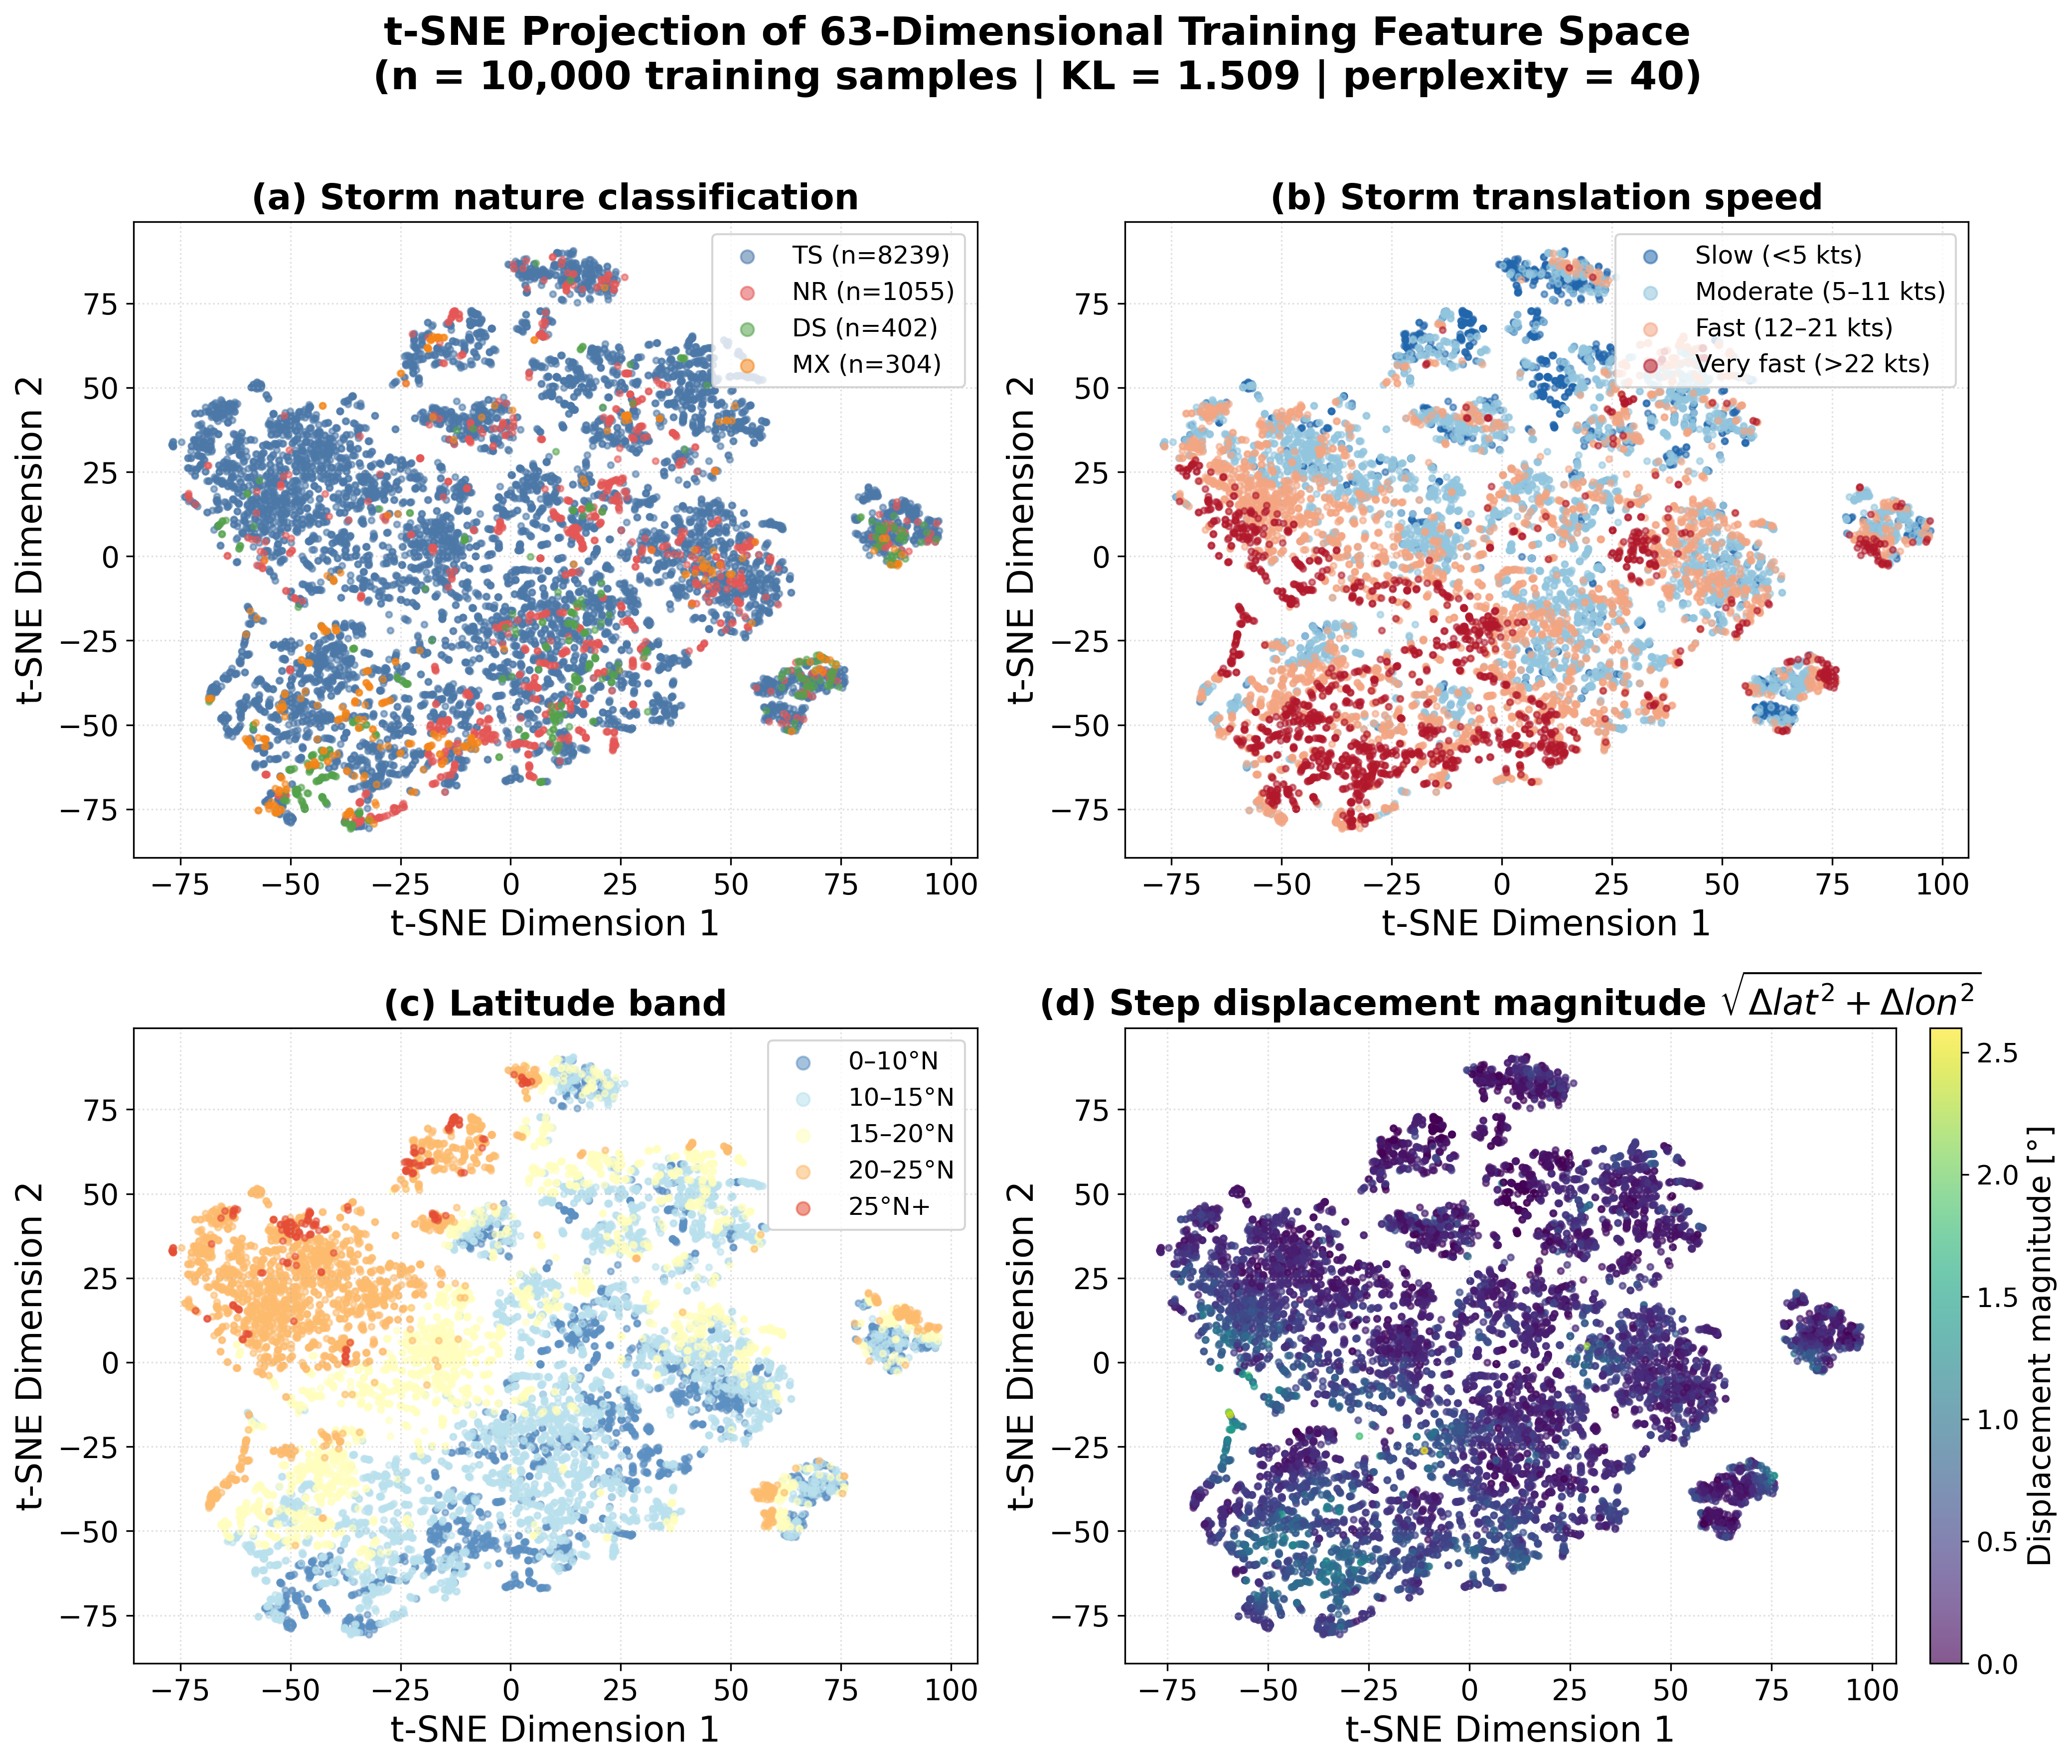
\includegraphics[width=0.98\textwidth]{fig01tsne}
\caption{t-SNE projection \citep{maaten2008tsne} of the 63-dimensional feature
space ($n=10{,}000$ training samples, held-out seed 0). Colouring by independent
meteorological attributes. Coherent separation indicates that the engineered
features encode physically distinct regimes, which is the premise of the
subset-expert design.}
\label{fig:tsne}
\end{figure}




\subsection{Genesis-window selection}
\label{sec:window}
The choice of genesis window trades training-set size against observational
quality. We evaluated three candidates, 1940--2024, 1979--2024, and 1990--2024,
on nine development seeds using a simple LightGBM baseline. Because both
\ibtracs{} and \era{} quality improve substantially once satellite observation
begins, and because pre-1979 records show near-total missingness in the wind
observations used for intensity estimation, a naive comparison risks confounding
``more training data'' with ``easier test set''. We therefore added a fixed-test
control in which models trained on each candidate window are all evaluated on one
common modern holdout drawn from 1990--2024 genesis, with the same test storms
excluded from every training set.

Table~\ref{tab:window} gives both comparisons. The wide window wins at every
horizon under the fixed-test control, so its advantage is not merely a
test-composition artefact. The size of that advantage is nonetheless strongly
horizon-dependent: at 3\,h the raw gap of 0.90\,km falls to 0.18\,km once test
composition is held fixed, whereas at 24 and 48\,h gaps of 7.9 and 17.7\,km
persist. We attribute this to storm \emph{position} records remaining comparatively
reliable across eras even where wind and intensity observations are sparse, which
is the relevant consideration because track geometry, not intensity, is the
target variable here. We accordingly lock 1940--2024 for all subsequent
modelling.

\begin{table}[ht]
\centering
\small
\begin{tabular}{@{}lrrrr@{}}
\toprule
Training window & 3\,h & 12\,h & 24\,h & 48\,h \\
\midrule
\multicolumn{5}{@{}l}{\textit{Each window on its own test split}}\\
\textbf{1940--2024} & \textbf{5.24} & \textbf{36.19} & \textbf{99.77} & \textbf{244.92} \\
1979--2024          & 6.13 & 44.04 & 112.38 & 271.40 \\
1990--2024          & 6.14 & 44.11 & 108.12 & 261.58 \\
\midrule
\multicolumn{5}{@{}l}{\textit{Fixed common modern holdout}}\\
\textbf{1940--2024} & \textbf{5.96} & \textbf{39.42} & \textbf{100.18} & \textbf{243.86} \\
1979--2024          & 6.07 & 42.24 & 103.86 & 249.82 \\
1990--2024          & 6.14 & 44.11 & 108.12 & 261.58 \\
\bottomrule
\end{tabular}
\caption{Genesis-window comparison, mean test median error in km over nine
development seeds with a simple LightGBM baseline. The upper block lets each
window use its own test split; the lower block trains on each window and
evaluates all three models on one common 1990--2024 genesis holdout.}
\label{tab:window}
\end{table}

% =============================================================================
\section{On Test-Set Leakage: A Methodological Note}
\label{sec:leakage}
% =============================================================================
During initial development, successive architecture revisions, which we refer to
internally as Phases~1 through~3, were evaluated on a single fixed
train/validation/test split. The decision to advance from one phase to the next
was taken by inspecting per-horizon performance gaps on that test set and
introducing targeted fusion-path additions intended to close them. No individual
test observation was used to fit any model parameter. Nevertheless this
iterative, human-guided design loop constitutes test-set leakage: the
architecture itself was shaped by repeated exposure to test-set feedback, which
invalidates the resulting held-out estimate as a measure of
generalisation~\citep{cawley2010}.

We detected the pattern by auditing, for each architectural decision point, which
data partition had informed it. Within-run decisions, namely fusion-path
selection and non-negative least squares weight fitting, proved to be properly
restricted to the validation partition. The \emph{cross-run} decision to advance
from one phase to the next, however, had been made by inspecting test-set rank
tables. The empirical symptom was unambiguous: an architecture that appeared to
win at every horizon on the original split did not reproduce that sweep on
independent fresh splits.

\textbf{Correction.} We adopted a strict two-tier seed protocol. Nine
\emph{development} seeds, $\{3,4,5,6,8,9,10,11,14\}$, carry every architectural and
fusion-path decision; during this stage the corresponding held-out partition is
neither generated nor examined. Nine \emph{held-out} seeds,
$\{0,1,2,7,13,99,123,2024,2026\}$, were generated once and evaluated exactly once,
after the architecture was frozen. Architectural convergence is verified by
confirming that development-seed and held-out-seed results agree, reported in
Section~\ref{sec:heldout}, rather than by any further tuning against held-out
performance.

We report this process transparently for two reasons. Iterative test-set
inspection is, in our reading, a common and under-scrutinised risk in
ensemble-based forecasting benchmarks. And our own uncorrected results, which
appeared to show the proposed ensemble winning at every horizon, failed to
replicate, which makes the risk concrete rather than hypothetical.

% =============================================================================
\section{Methodology}
\label{sec:methods}
% =============================================================================


\subsection{Baseline systems}
Seven baselines are benchmarked alongside the proposed ensemble. The
\textbf{Stacking Ensemble} combines Random Forest, XGBoost, and LightGBM base
learners through a Ridge-penalised, cross-validated linear meta-learner. The
\textbf{Persistence Residual Cascade (PRC)} corrects a naive persistence
extrapolation with a dedicated LightGBM residual model fitted in kilometre space
and mapped back to degrees. \textbf{Random Forest}~\citep{breiman2001rf},
\textbf{LightGBM}~\citep{ke2017lightgbm}, \textbf{XGBoost}~\citep{chen2016xgboost},
and \textbf{CatBoost}~\citep{prokhorenkova2018catboost} are included as individual
learners. \textbf{CB+MotionNN} corrects a CatBoost predictor with a 64-32-16
feedforward network operating on kinematic residual features.

\subsection{Proposed architecture: SECE Phase~3}
For each forecast horizon, \sece{} constructs four physics-informed feature
subsets. At 3\,h these are position, motion, environ, and the full feature set;
at 12, 24, and 48\,h they are motion, physics, environ, and full. Each subset is
modelled independently by four tree algorithms, namely CatBoost, XGBoost,
LightGBM, and Random Forest, giving sixteen subset-level models per horizon,
which are fused by non-negative least squares into a single subset-consensus
signal with separate weights for the latitude and longitude components.

That subset-consensus signal is then combined with the seven baseline
predictions, the ``champion'' pool, in a second-stage non-negative least squares
fusion. A horizon-specific set of fusion-path candidates is constructed, listed
in Table~\ref{tab:fusion}, and a hard validation-best router selects, per seed,
whichever candidate achieves the lowest validation median error. The selected
candidate's predictions are what we report. Both the router selection and all
weight fitting are restricted to the validation partition, in keeping with
Section~\ref{sec:leakage}. Fig.~\ref{fig:arch} summarises the pipeline.

\begin{figure}[ht]
\centering
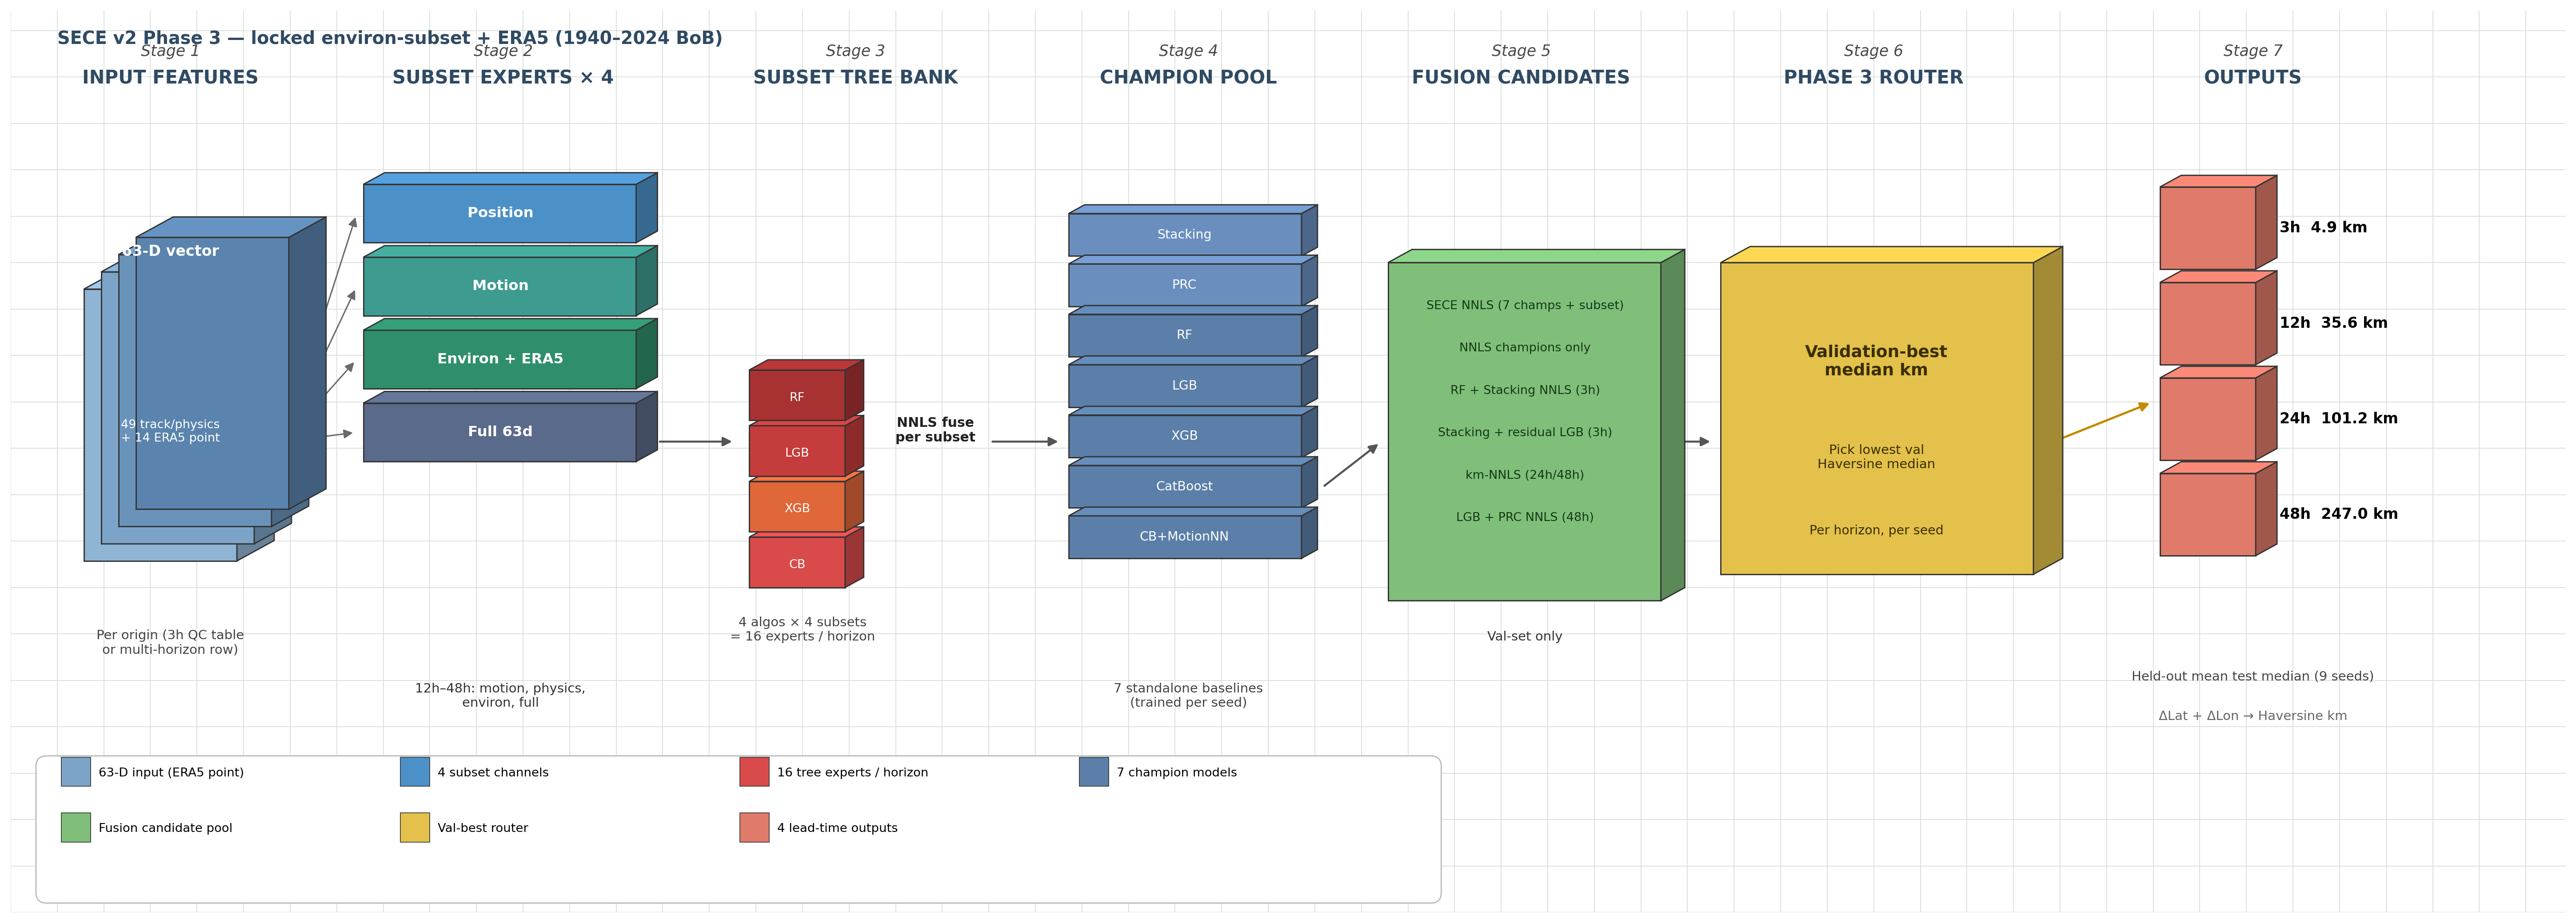
\includegraphics[width=0.98\textwidth]{fig02arch}
\caption{Locked SECE v2 Phase~3 pipeline. Input is a 63-dimensional vector
(49 track/physics features plus 14 point \era{} fields). Four subset experts,
each an NNLS fusion of four tree algorithms, enter a champion pool with seven
standalone baselines; a validation-only router selects the fusion candidate with
the lowest validation median error at each horizon.}
\label{fig:arch}
\end{figure}


\begin{table}[ht]
\centering
\small
\begin{tabular}{@{}ll@{}}
\toprule
Horizon & Candidate fusion paths \\
\midrule
3\,h  & \sece{} NNLS full pool; NNLS champions only; RF$+$Stacking NNLS; \\
      & Stacking with LightGBM residual correction \\
12\,h & \sece{} NNLS full pool; NNLS champions only \\
24\,h & \sece{} NNLS full pool; NNLS champions only; \\
      & kilometre-space NNLS over champions, persistence-anchored \\
48\,h & as 24\,h, plus LightGBM$+$PRC NNLS and LightGBM$+$PRC kilometre-NNLS \\
\bottomrule
\end{tabular}
\caption{Horizon-specific fusion candidates available to the validation-only
router. The kilometre-space variant fits weights on persistence-anchored
residuals scaled to kilometres and then adds the persistence term back.}
\label{tab:fusion}
\end{table}

\textbf{The environ expert.} Rather than folding the 14 \era{} features into
existing subsets, we allocate them, together with the native environmental fields
for distance to land, landfall state, and storm speed and direction, to a
dedicated environ subset with its own four-algorithm expert pool. This choice was
made over three tested alternatives, namely \era{} features added directly to
existing point-feature subsets and \era{} spatial-patch features at 5$^\circ$ and
3$^\circ$, on the basis of the best balanced performance across all four horizons
reported in Section~\ref{sec:ablation}. It also admits a more direct mechanistic
reading, since atmospheric information receives explicit ensemble representation
rather than competing for splits inside a larger undifferentiated subset.

\subsection{Training protocol}
All tree models use the settings in Table~\ref{tab:hyp}, applied uniformly across
every system so that measured differences reflect architecture rather than
tuning budget~\citep{grinsztajn2022tree}. Early stopping is disabled for the tree
learners.

\begin{table}[ht]
\centering
\begin{tabular}{@{}p{0.42\textwidth}p{0.52\textwidth}@{}}
\toprule
Component & Setting \\
\midrule
Locked architecture & SECE v2 Phase 3 + point ERA5 + environ expert \\
Genesis window & 1940--2024 IBTrACS NI + ERA5 point features \\
Held-out seeds & 0, 1, 2, 7, 13, 99, 123, 2024, 2026 \\
Development seeds (architecture lock only) & 3, 4, 5, 6, 8, 9, 10, 11, 14 \\
Split & storm-wise 70:15:15, seed-specific \\
3\,h SECE subsets & position, motion, environ, full \\
12/24/48\,h SECE subsets & motion, physics, environ, full \\
Subset tree algorithms & CatBoost, XGBoost, LightGBM, Random Forest $\times$ each subset \\
Subset experts & 4 subsets $\times$ 4 algorithms $=$ 16 trees, NNLS-fused to 1 subset signal \\
Champion / standalone bases & Stacking, PRC, RF, LightGBM, XGBoost, CatBoost, CB+MotionNN \\
NNLS full pool & 7 champions + 1 subset-NNLS signal (degree space, separate lat/lon weights) \\
Router (Phase 3) & hard val-best: lowest validation median km \\
3\,h extra fusion candidates & SECE NNLS full, NNLS champions, RF+STK NNLS, STK+residual LGB \\
24\,h extra fusion candidates & SECE NNLS full, NNLS champions, km-NNLS (champions, persistence-anchored) \\
48\,h extra fusion candidates & as 24\,h plus LGB+PRC NNLS and LGB+PRC km-NNLS \\
Global learning rate & 0.01 \\
Tree $n_{\mathrm{estimators}}$ (RF/XGB/LGB/CB) & 300 \\
Tree max depth / CatBoost depth & 6 \\
LightGBM \texttt{num\_leaves} & 63 \\
XGBoost subsample / colsample by tree & 0.8 / 0.8 \\
Stacking STK\_N (RF+XGB+LGB Ridge) & 150 \\
MotionNN & MLP 64-32-16, ReLU, lr 0.01, max\_iter 100, early stopping \\
PRC & persistence displacement + LightGBM residual in km, mapped back to degrees \\
km-NNLS & NNLS on (pred$-$persist)$\times$(111,111) km, then add persist \\
ERA5 environ keys & $u,v$ at 850/500/200\,hPa, MSL, SST, steer $u,v$, shear $u,v$, shear magnitude, SST missing flag \\
Environ subset also includes & DIST2LAND, LANDFALL, NEWDELHI, STORM\_SPEED, STORM\_DIR + ERA5 keys \\
Not evaluated on held-out & CNN-GRU, BLSTM, other deep models \\
\bottomrule
\end{tabular}
\caption{Locked architecture and hyperparameters from
\texttt{02\_architecture\_hyperparameters.csv}, applied uniformly across systems
unless noted. CNN-GRU and BLSTM were not re-trained on this held-out protocol.}
\label{tab:hyp}
\end{table}

\subsection{Evaluation metric and statistical testing}
The primary metric is median great-circle (Haversine) error in kilometres between
predicted and verified storm position, computed per test storm and
aggregated~\citep{sinnott1984}. The median rather than the mean
is used because per-storm error distributions are strongly right-skewed, so a
mean would be dominated by a small number of recurving or rapidly accelerating
systems.

For the final held-out evaluation we additionally report 95\% confidence
intervals on the pooled median obtained from 10{,}000 storm-level bootstrap
resamples~\citep{efron1979}, and paired Wilcoxon
signed-rank tests comparing \sece{} against each of the seven baselines on
matched per-storm median errors~\citep{wilcoxon1945}. Resampling
and pairing are performed at storm level, not sample level, so that the unit of
statistical independence matches the unit of the split. Bonferroni correction is
applied across the seven simultaneous
comparisons~\citep{bonferroni1936}, giving an adjusted threshold of
$\alpha = 0.05/7 \approx 0.0071$.

\subsection{Systems excluded from the held-out table}
\label{sec:dlscope}
Before the \era{}-augmented design was frozen we trained CNN-GRU and
bidirectional LSTM~\citep{lian2020novel,graves2005blstm} alongside the tree
learners on storm-wise development splits, using the same fixed budget philosophy
as the locked tree protocol (300 estimators or epochs, learning rate 0.01, no
architecture-specific hyperparameter search). In those exploratory runs---track-only
features first, then informal checks after \era{} was added---both recurrent
models repeatedly ranked below Random Forest, stacking, and gradient boosting at
3, 12, and 24\,h, with short-lead errors closer to persistence-scale displacement
than the sub-6\,km medians the trees achieved. That pattern is consistent with
\citet{grinsztajn2022tree} on tabular cyclone features at basin sample sizes. We
therefore scoped the leakage-corrected held-out confirm to the eight tree and
hybrid systems already in the production pipeline (Table~\ref{tab:heldout}) rather
than porting sequence training to nine fresh held-out seeds and a 48\,h head.
CNN-GRU and BLSTM are absent from every held-out result and figure reported here.
% =============================================================================
\section{Results}
\label{sec:results}
% =============================================================================


\subsection{Development-phase ablation}
\label{sec:ablation}
Table~\ref{tab:abl} reports, for each feature configuration, the number of
development seeds out of nine on which \sece{} achieved the lowest median error
among all eight systems, together with its mean median error across those seeds.

Two findings motivate the locked architecture. First, \era{} point features
substantially reduce \sece{}'s mean error at 48\,h, from 250.26 to 246.80\,km,
with 8 of 9 development seeds improving. This establishes that atmospheric
information carries genuine, exploitable signal at long lead times rather than
merely adding dimensionality. Second, allocating those features to a dedicated
environ expert instead of embedding them in existing subsets improves 24\,h
performance specifically, raising rank-1 frequency from 2/9 to 3/9 and reducing
mean error from 99.86 to 99.43\,km; 24\,h was precisely the horizon at which the
plain point-\era{} configuration was weakest.

The same table records a cost that we report rather than suppress. At 3\,h the
track-only configuration retains the lowest mean error, 4.84 against 4.93\,km, so
\era{} does not help uniformly across horizons. The short-range gain from \era{}
in this architecture is expressed as rank stability rather than as a lower mean.

Spatial-patch features improved short-range rank-1 frequency, reaching 7/9 at both
3 and 12\,h, but showed no consistent advantage over the environ-expert
configuration at 24 or 48\,h, where means fall within roughly 0.4\,km of each
other, inside the seed-to-seed noise floor (Fig.~\ref{fig:ablation}). We therefore
did not adopt spatial-patch features into the locked architecture, and report this
as a negative result.

\begin{table}[ht]
\centering
\footnotesize
\begin{tabular}{@{}lcccc@{}}
\toprule
Configuration & 3\,h & 12\,h & 24\,h & 48\,h \\
\midrule
Track-only (no \era{})          & 5/9, 4.84 & 3/9, 35.48 & 3/9, 100.48 & 0/9, 250.26 \\
$+$ \era{} point features       & 5/9, 4.93 & 7/9, 35.59 & 2/9, \phantom{0}99.86 & 1/9, 246.80 \\
\textbf{$+$ environ expert (locked)} & \textbf{5/9, 4.93} & \textbf{6/9, 35.56} & \textbf{3/9, \phantom{0}99.43} & \textbf{2/9, 246.94} \\
$+$ spatial patch (5$^\circ$)   & 7/9, 4.93 & 7/9, 35.56 & 1/9, \phantom{0}99.74 & 1/9, 246.55 \\
$+$ spatial patch (3$^\circ$)   & 7/9, 4.93 & 7/9, 35.66 & 2/9, \phantom{0}99.42 & 3/9, 247.00 \\
\midrule
Held-out confirm (locked)       & 6/9, 4.90 & 6/9, 35.63 & 2/9, 101.21 & 1/9, 246.99 \\
\bottomrule
\end{tabular}
\caption{Development-seed ablation over nine development seeds. Each cell gives
the \sece{} rank-1 count out of nine, then the mean median error in km. The locked
configuration is in bold. The final row is the independent held-out confirm on
disjoint seeds, included here only to show tier agreement.}
\label{tab:abl}
\end{table}


\begin{figure}[ht]
\centering
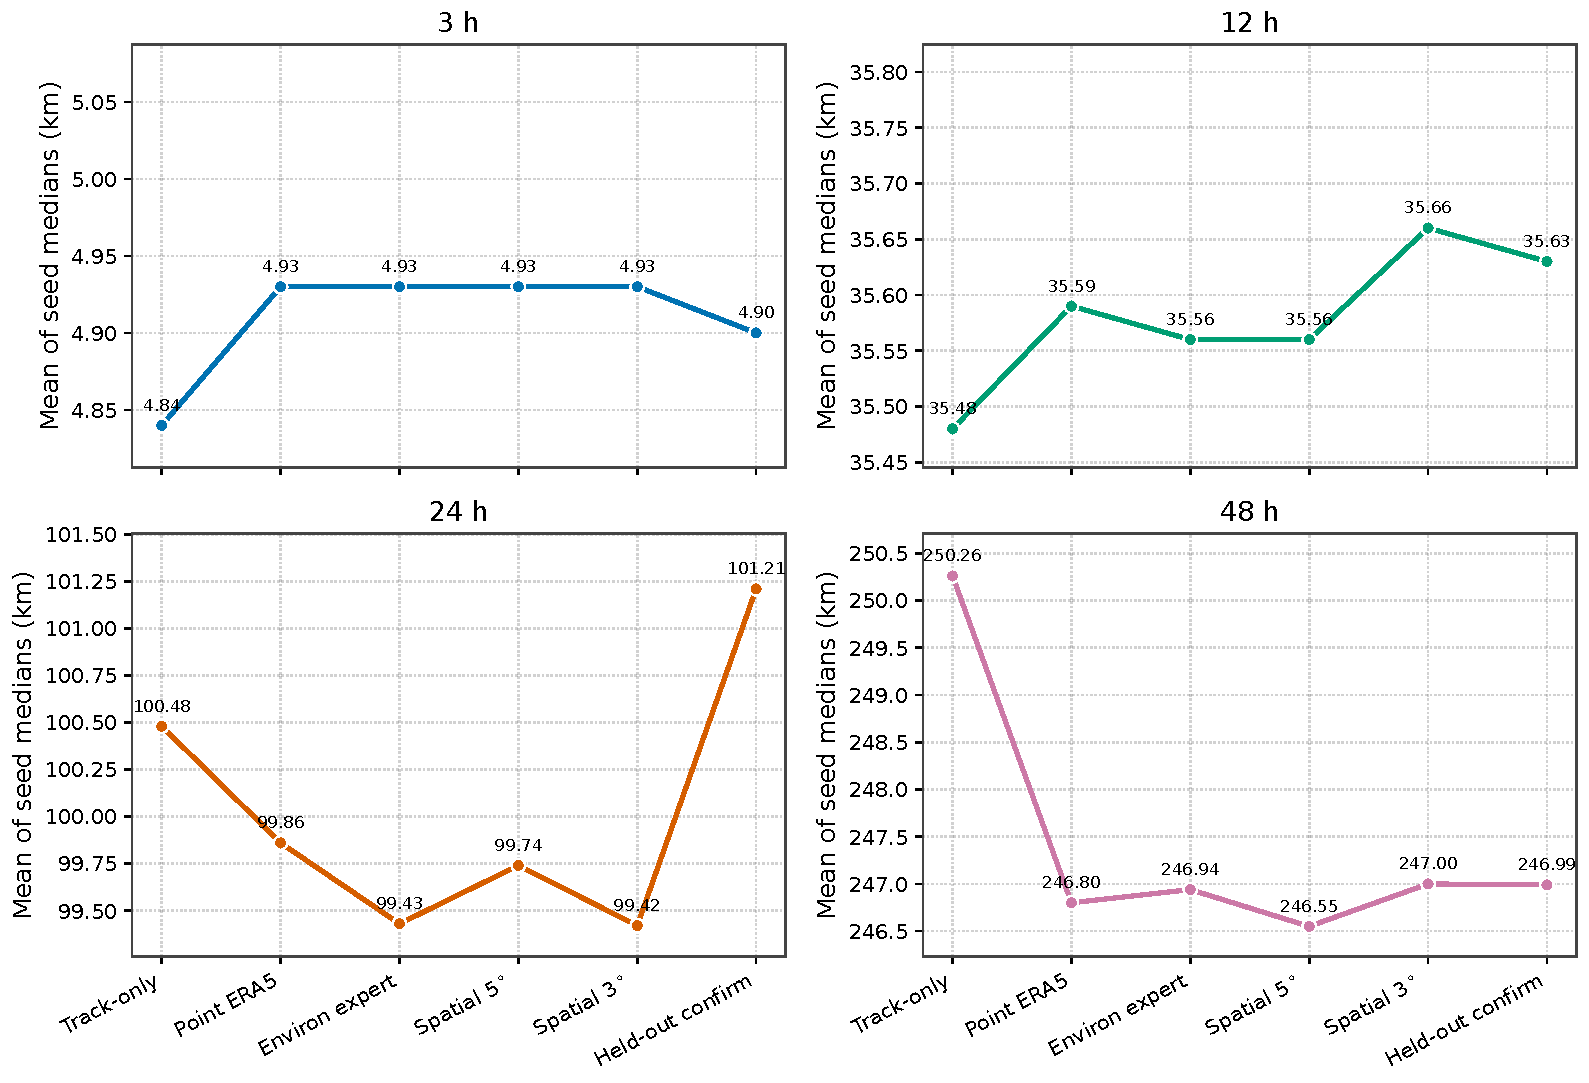
\includegraphics[width=0.98\textwidth]{fig03ablation}
\caption{Development ablation trend from
\texttt{full\_experiment\_summary\_table.csv}. The $y$-axis is the mean of SECE
test medians across nine seeds (km). Configurations on the $x$-axis are sequential
interventions on the development seeds except the last point, which is the
independent held-out confirm on nine disjoint seeds (not a sixth architecture).
Each panel uses its own vertical scale so that 3\,h changes of a few tenths of a
kilometre remain visible. Point \era{} helps at 48\,h; the environ expert is the
locked 24\,h compromise; spatial 5$^\circ$/3$^\circ$ patches do not justify
adoption over the environ expert.}
\label{fig:ablation}
\end{figure}

Fig.~\ref{fig:ablation} shows the same mean-median series as a trend across configurations so that the horizon at which each intervention helps, or fails to help, is visible at a glance.

\subsection{Held-out evaluation}
\label{sec:heldout}
Table~\ref{tab:heldout} reports pooled median errors and bootstrap confidence
intervals for all eight systems at all four horizons, over 34{,}114 test samples
at 3\,h and 21{,}442 at the longer horizons.

At 3\,h \sece{} leads with 4.895\,km, ahead of Random Forest at 4.927\,km and the
Stacking Ensemble at 4.945\,km, with a clear gap to the remaining five systems. At
12\,h \sece{} again leads with 35.538\,km against 36.146\,km for stacking. At
24\,h the ordering changes: stacking and XGBoost take the top two point estimates,
100.771 and 101.029\,km, with \sece{} third at 101.186\,km. At 48\,h XGBoost and
PRC lead with 242.702 and 243.229\,km against 246.331\,km for \sece{}. In both
long-lead cases the confidence intervals overlap almost entirely, which is why the
paired tests rather than the point estimates carry the inferential weight.

Table~\ref{tab:wilcox} gives those tests in full, with Bonferroni-adjusted
$p$-values and the rank-biserial correlation as an effect size. At 3 and 12\,h all
seven comparisons are significant after correction, so \sece{} beats every
baseline at both short horizons. At 24\,h only CatBoost and CB+MotionNN remain
significant; Random Forest is significant raw but not after correction, and
stacking, PRC, LightGBM, and XGBoost are not significant by either standard. At
48\,h only CatBoost remains significant, with stacking and CB+MotionNN
significant raw but not after correction.

The effect-size column carries an important detail. Every rank-biserial
correlation in the table is negative, which under our sign convention means
\sece{} holds the lower per-storm error in the paired comparison. Consequently
\sece{} is never significantly \emph{worse} than any baseline at any horizon; at
long lead the correct statement is parity, not defeat. The magnitudes also make
the horizon dependence visible: against stacking the effect size falls from
$-0.208$ at 3\,h to $-0.071$ at 24\,h, and against XGBoost from $-0.993$ to
$-0.003$ at 48\,h.

\begin{table}[ht]
\centering
\footnotesize
\begin{tabular}{@{}llrr@{}}
\toprule
Horizon & System & Median (km) & 95\% CI \\
\midrule
\multirow{8}{*}{3\,h}
 & \textbf{\sece{} v2 Phase~3} & \textbf{4.895} & [4.714, 5.079] \\
 & Random Forest               & 4.927 & [4.734, 5.125] \\
 & Stacking Ensemble           & 4.945 & [4.763, 5.123] \\
 & CB$+$MotionNN               & 5.813 & [5.701, 5.928] \\
 & LightGBM                    & 6.026 & [5.889, 6.168] \\
 & XGBoost                     & 6.411 & [6.243, 6.580] \\
 & CatBoost                    & 8.479 & [8.284, 8.691] \\
 & PRC                         & 8.872 & [8.707, 9.058] \\
\midrule
\multirow{8}{*}{12\,h}
 & \textbf{\sece{} v2 Phase~3} & \textbf{35.538} & [34.208, 36.925] \\
 & Stacking Ensemble           & 36.146 & [34.744, 37.701] \\
 & Random Forest               & 36.901 & [35.525, 38.323] \\
 & LightGBM                    & 36.928 & [35.498, 38.338] \\
 & XGBoost                     & 36.947 & [35.531, 38.416] \\
 & PRC                         & 37.177 & [35.704, 38.527] \\
 & CB$+$MotionNN               & 37.413 & [36.047, 38.949] \\
 & CatBoost                    & 42.028 & [40.381, 43.656] \\
\midrule
\multirow{8}{*}{24\,h}
 & Stacking Ensemble           & 100.771 & [96.887, 104.703] \\
 & XGBoost                     & 101.029 & [96.932, 105.286] \\
 & \textbf{\sece{} v2 Phase~3} & \textbf{101.186} & [97.301, 104.808] \\
 & LightGBM                    & 101.632 & [97.778, 105.589] \\
 & PRC                         & 101.941 & [98.131, 105.824] \\
 & Random Forest               & 103.511 & [99.652, 107.437] \\
 & CB$+$MotionNN               & 104.034 & [100.239, 108.074] \\
 & CatBoost                    & 107.191 & [102.555, 111.839] \\
\midrule
\multirow{8}{*}{48\,h}
 & XGBoost                     & 242.702 & [232.596, 255.403] \\
 & PRC                         & 243.229 & [231.650, 255.158] \\
 & LightGBM                    & 245.975 & [234.926, 257.214] \\
 & Stacking Ensemble           & 245.977 & [235.938, 257.183] \\
 & \textbf{\sece{} v2 Phase~3} & \textbf{246.331} & [235.541, 257.614] \\
 & CB$+$MotionNN               & 249.678 & [238.972, 261.153] \\
 & Random Forest               & 251.305 & [240.752, 262.324] \\
 & CatBoost                    & 254.862 & [242.991, 267.797] \\
\bottomrule
\end{tabular}
\caption{Held-out test performance: pooled median great-circle error in km with
95\% bootstrap confidence interval from 10{,}000 storm-level resamples. Nine
held-out seeds pooled; 442 distinct storm identifiers. Eight tree/hybrid systems
only; CNN-GRU and BLSTM omitted (section~\ref{sec:dlscope}).}
\label{tab:heldout}
\end{table}

\begin{table}[ht]
\centering
\footnotesize
\setlength{\tabcolsep}{5pt}
\begin{tabular}{@{}lrrrrrrrr@{}}
\toprule
& \multicolumn{2}{c}{3\,h} & \multicolumn{2}{c}{12\,h}
& \multicolumn{2}{c}{24\,h} & \multicolumn{2}{c}{48\,h} \\
\cmidrule(lr){2-3}\cmidrule(lr){4-5}\cmidrule(lr){6-7}\cmidrule(lr){8-9}
Baseline & $p$ & $r$ & $p$ & $r$ & $p$ & $r$ & $p$ & $r$ \\
\midrule
Stacking Ensemble & \textbf{0.0016} & $-0.208$ & \textbf{0.0014} & $-0.210$ & 1.000 & $-0.071$ & 0.262$^{\dagger}$ & $-0.114$ \\
Random Forest     & \textbf{0.0272} & $-0.164$ & \textbf{$1.1\times10^{-5}$} & $-0.263$ & 0.0737$^{\dagger}$ & $-0.140$ & 0.704 & $-0.090$ \\
LightGBM          & \textbf{$<10^{-6}$} & $-0.970$ & \textbf{$<10^{-6}$} & $-0.306$ & 1.000 & $-0.044$ & 1.000 & $-0.068$ \\
XGBoost           & \textbf{$<10^{-6}$} & $-0.993$ & \textbf{$<10^{-6}$} & $-0.364$ & 1.000 & $-0.046$ & 1.000 & $-0.003$ \\
PRC               & \textbf{$<10^{-6}$} & $-1.000$ & \textbf{$<10^{-6}$} & $-0.394$ & 0.898 & $-0.084$ & 1.000 & $-0.005$ \\
CatBoost          & \textbf{$<10^{-6}$} & $-1.000$ & \textbf{$<10^{-6}$} & $-0.806$ & \textbf{$<10^{-6}$} & $-0.450$ & \textbf{$<10^{-6}$} & $-0.352$ \\
CB$+$MotionNN     & \textbf{$<10^{-6}$} & $-0.833$ & \textbf{$<10^{-6}$} & $-0.443$ & \textbf{$1\times10^{-5}$} & $-0.265$ & 0.262$^{\dagger}$ & $-0.114$ \\
\bottomrule
\end{tabular}
\caption{Paired Wilcoxon signed-rank tests of \sece{} against each baseline on 442
matched per-storm medians, reporting the Bonferroni-adjusted $p$-value and the
rank-biserial correlation $r$ as an effect size. Bold marks a significant \sece{}
advantage at the adjusted threshold $\alpha \approx 0.0071$; a dagger marks
significance before correction only. Every $r$ is negative, meaning \sece{} holds
the lower per-storm error, so no baseline is significantly better than \sece{} at
any horizon. The collapse of $|r|$ from 3 to 48\,h is the quantitative signature
of the horizon dependence discussed in Section~\ref{sec:discussion}.}
\label{tab:wilcox}
\end{table}

Pooled medians summarise central tendency but hide how often each system wins
outright. Table~\ref{tab:rank1} therefore counts, per horizon, how many of the
nine held-out seeds each system led. The pattern reinforces the significance
tests: \sece{} takes 6 of 9 seeds at both 3 and 12\,h, but only 2 of 9 at 24\,h
and 1 of 9 at 48\,h, where PRC and XGBoost lead more often. A system can hold the
best pooled median while winning a minority of seeds, and both views are needed to
describe long-lead behaviour honestly.

\begin{table}[ht]
\centering
\small
\begin{tabular}{@{}ll@{}}
\toprule
Horizon & Seeds led (out of nine) \\
\midrule
3\,h  & \sece{} 6, Random Forest 2, Stacking 1 \\
12\,h & \sece{} 6, Stacking 3 \\
24\,h & Stacking 3, \sece{} 2, LightGBM 2, XGBoost 2 \\
48\,h & PRC 4, XGBoost 3, \sece{} 1, Stacking 1 \\
\bottomrule
\end{tabular}
\caption{Number of held-out seeds, out of nine, on which each system achieved the
lowest test median error. Systems not listed for a horizon led on no seed.}
\label{tab:rank1}
\end{table}

Fig.~\ref{fig:bench} places the eight systems in the mean-error versus
accuracy-index plane at all four horizons (mean on the horizontal axis; medians
in Table~\ref{tab:heldout}). At 3 and 12\,h the leading systems separate visibly
from the remainder; at 24 and 48\,h they collapse onto a common cluster.

\begin{figure}[ht]
\centering
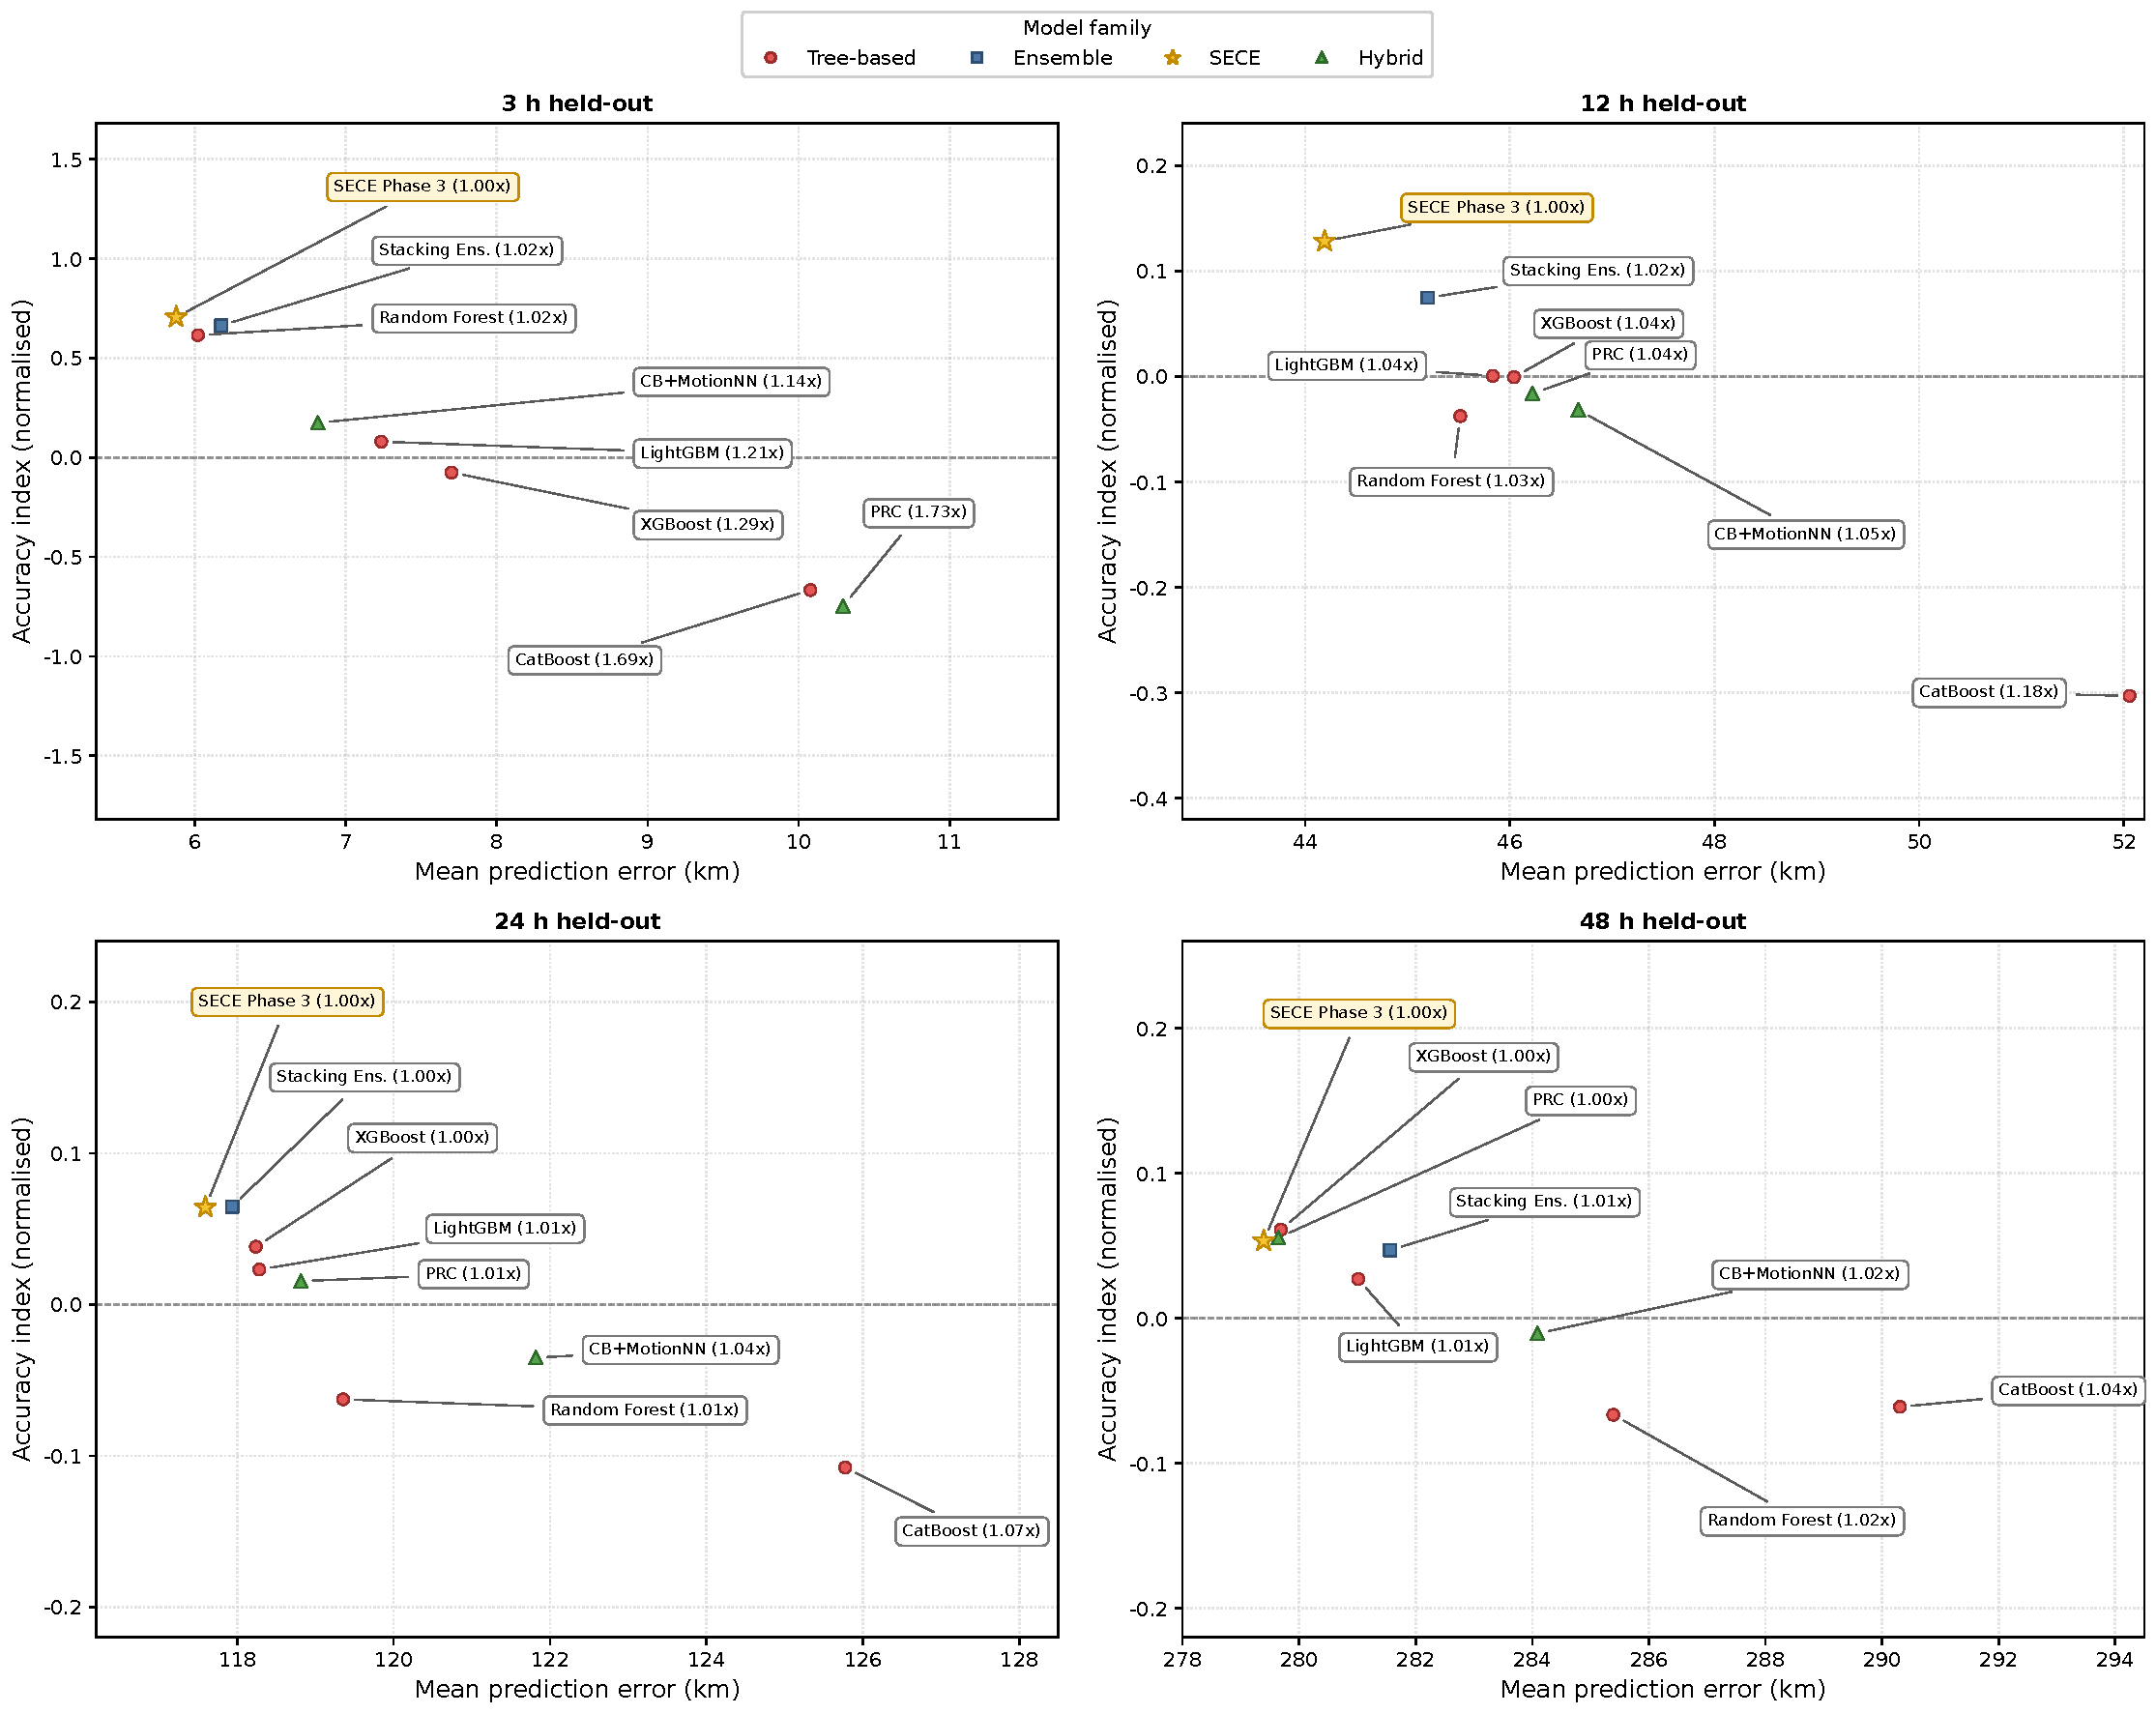
\includegraphics[width=0.98\textwidth]{fig04bench4h}
\caption{Held-out four-horizon benchmark for the eight locked systems.
Each point is computed from the pooled nine-seed held-out prediction export
(\texttt{results/sece\_era5\_environ\_heldout/task\_a\_test\_predictions/}),
audited in \texttt{benchmark\_*h\_heldout\_stats.json}. The horizontal axis is
\emph{mean} great-circle error (km) over all scored test origins; parenthetical
multipliers are that system's mean divided by the SECE mean. The vertical axis is
an accuracy index derived from \emph{median} error, normalised so that the
tree-family median sits at zero. Table~\ref{tab:heldout} reports the corresponding
medians with bootstrap confidence intervals. Mean and median therefore answer
different questions and are not interchangeable.}
\label{fig:bench}
\end{figure}


\subsection{Per-storm ERA5 contribution at long horizons}
\label{sec:diag}
To characterise the distribution of \era{}'s benefit independently of the ensemble
machinery, we compare a single LightGBM model trained with and without \era{}
features, storm by storm, on a representative development seed with 88 test
storms. At 24\,h \era{} improves accuracy for 43 of 88 storms, or 48.9\%, with a
near-zero mean effect, indicating rough parity at this horizon for this simpler
model. At 48\,h it improves accuracy for 54 of 88 storms, or 61.4\%, with a median
per-storm improvement of 10.9\,km (Fig.~\ref{fig:era5hist}).

The benefit therefore strengthens with lead time. This is consistent with the
mechanistic expectation that a storm's own recent kinematic history becomes a
progressively weaker predictor of its future position, so large-scale steering
information becomes proportionally more
valuable~\citep{giffard2020tropical,goerss2004tropical}.

\begin{figure}[ht]
\centering
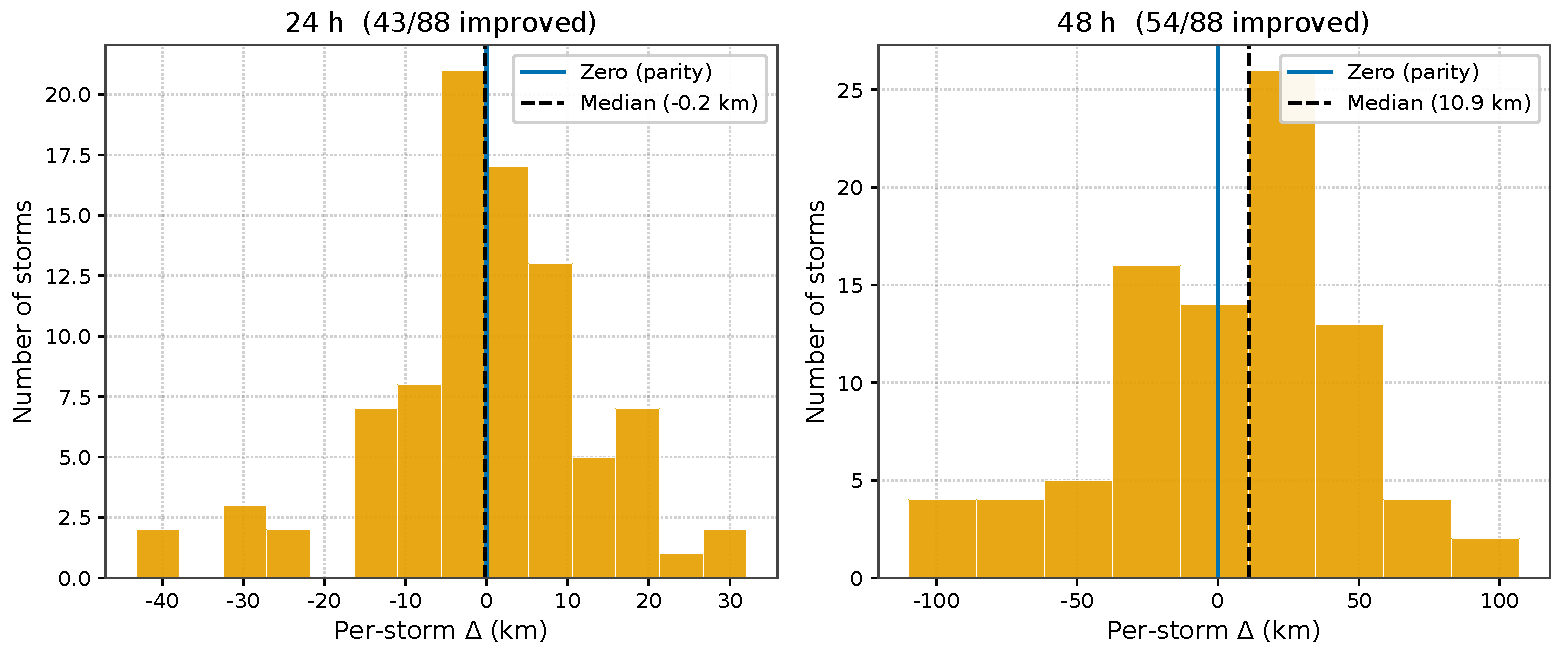
\includegraphics[width=0.98\textwidth]{fig05era5hist}
\caption{Per-storm LightGBM diagnostic comparing track-only error with
point-\era{} error on held-out seed 0
(\texttt{05\_seed0\_lgb\_era5\_vs\_trackonly\_per\_storm.csv}).
$\Delta$ is track-only median error minus \era{}-informed median error, so
positive values mean \era{} improved that storm. Blue: zero (parity); black
dashed: median $\Delta$. Panel titles report $n_{\mathrm{improved}}/n_{\mathrm{total}}$.
This is a single-model, single-seed diagnostic, not the full SECE stack.}
\label{fig:era5hist}
\end{figure}




\subsection{Feature importance within the environ expert}
\label{sec:fi}
Table~\ref{tab:fi} and Fig.~\ref{fig:featimp} report gain-based importance for the
environ-subset expert, from a diagnostic retrain on one held-out seed under the
locked LightGBM specification, averaged across the latitude and longitude output
heads. This is a single-seed tree-gain diagnostic, not a SHAP or multi-seed
attribution, and we present it only as an indication of which fields that
particular expert relies upon.

\begin{figure}[ht]
\centering
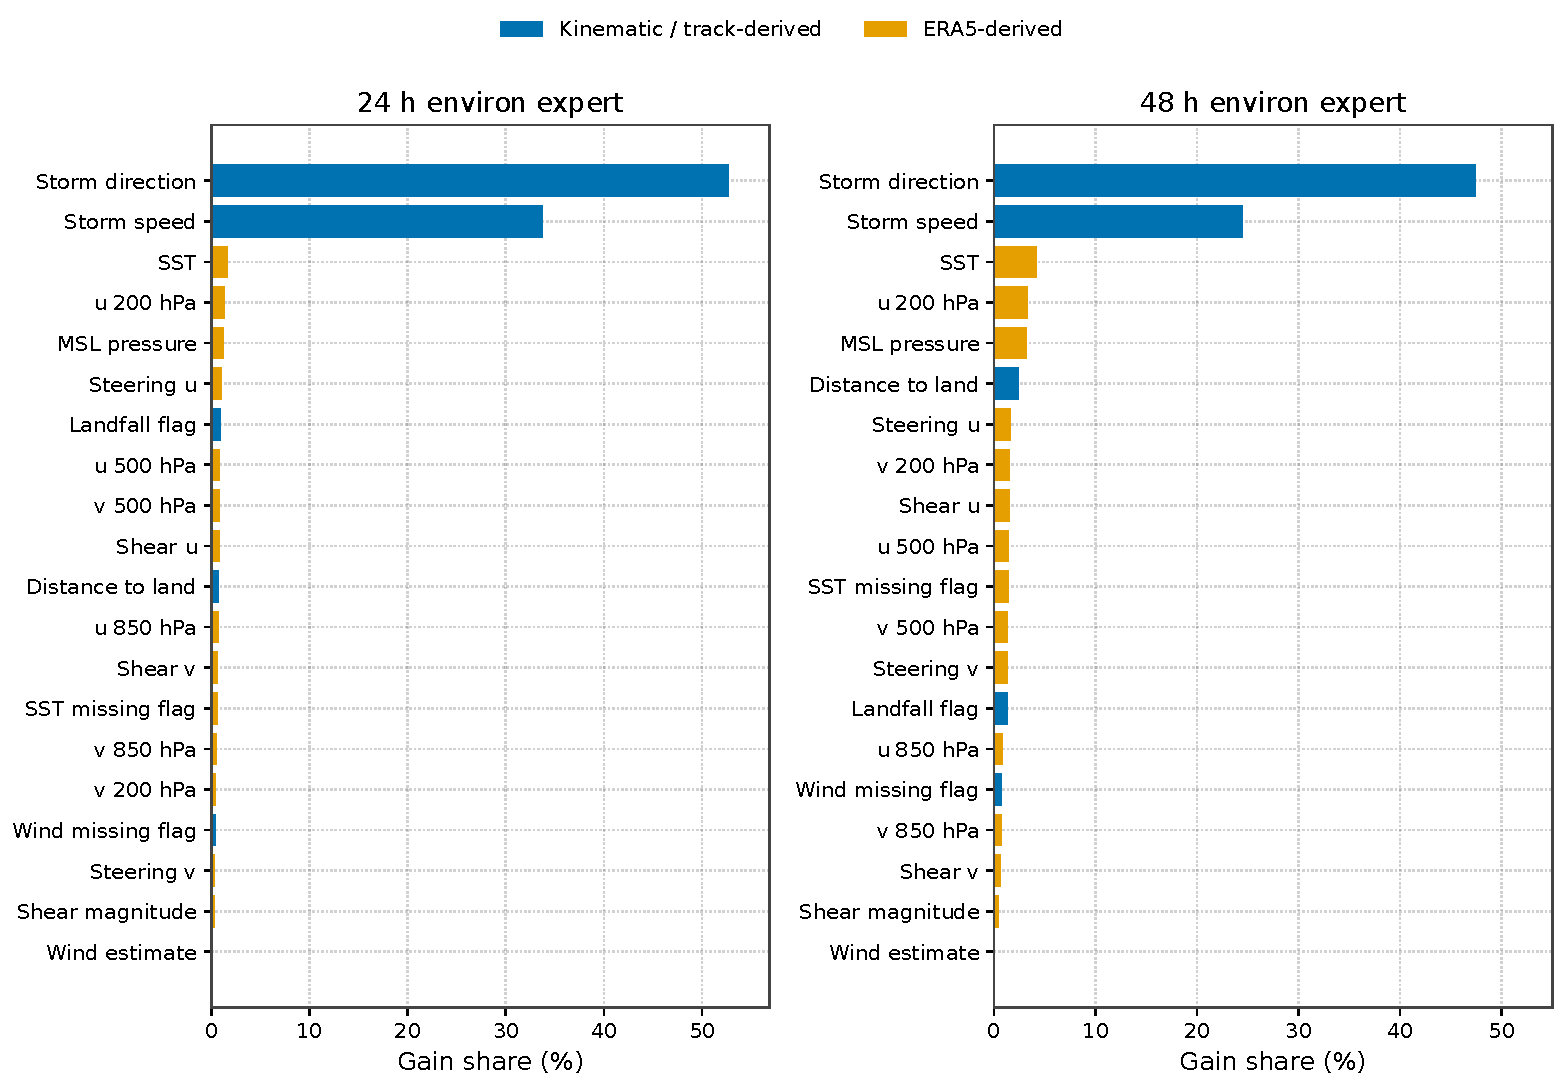
\includegraphics[width=0.98\textwidth]{fig06featimp}
\caption{LightGBM gain share for every feature in the environ-subset expert at
24 and 48\,h, from \texttt{04\_environ\_expert\_feature\_importance.csv}.
Blue: kinematic / track-derived features; orange: \era{}-derived features,
the colour convention used throughout this manuscript. Bars are sorted by gain
share. This is held-out seed 0 only, gain-based (not SHAP or permutation
importance), and environ-expert-only (not the full SECE stack).}
\label{fig:featimp}
\end{figure}


Two observations survive that caveat. First, kinematic features retain the
dominant share of gain even inside this \era{}-inclusive expert: storm direction
and speed are the two highest-ranked features at both horizons, which underscores
that atmospheric information supplements rather than displaces kinematic signal.
Second, every \era{} field's share of gain grows markedly from 24 to 48\,h, with
sea surface temperature rising from 1.66\% to 4.15\% and 200\,hPa zonal wind from
1.34\% to 3.32\%, which is an independent signature of the same lead-time
dependence found in Section~\ref{sec:diag}.

We deliberately do not interpret rank order within the shear and steering group.
Those components are mutually collinear by construction, since shear is defined as
a difference of the same wind levels that enter the steering term, so gain-based
importance may apportion credit arbitrarily among them. Dropping one wind level or
replacing the expert with ridge regression would remove the physical shear--steering
decomposition the environ subset is meant to preserve; grouped permutation or SHAP
tests would be needed for stable attribution within that block. Our claim is the
lead-time \emph{growth} of total \era{} gain (Section~\ref{sec:diag}), not the
within-group rank order.

\begin{table}[ht]
\centering
\footnotesize
\begin{tabular}{@{}lrr@{}}
\toprule
\era{} field & Share at 24\,h & Share at 48\,h \\
\midrule
Sea surface temperature (\texttt{sst}) & 0.0166 & 0.0415 \\
200\,hPa zonal wind (\texttt{u200})    & 0.0134 & 0.0332 \\
Mean sea level pressure (\texttt{msl}) & 0.0128 & 0.0323 \\
Steering wind, zonal (\texttt{steer\_u}) & 0.0101 & 0.0161 \\
500\,hPa zonal wind (\texttt{u500})    & 0.0086 & 0.0141 \\
500\,hPa meridional wind (\texttt{v500}) & 0.0085 & 0.0137 \\
Shear, zonal (\texttt{shear\_u})       & 0.0078 & 0.0152 \\
850\,hPa zonal wind (\texttt{u850})    & 0.0070 & 0.0084 \\
Shear, meridional (\texttt{shear\_v})  & 0.0067 & 0.0064 \\
SST imputation flag (\texttt{sst\_missing}) & 0.0067 & 0.0140 \\
850\,hPa meridional wind (\texttt{v850}) & 0.0048 & 0.0074 \\
200\,hPa meridional wind (\texttt{v200}) & 0.0044 & 0.0156 \\
Steering wind, meridional (\texttt{steer\_v}) & 0.0036 & 0.0135 \\
Shear magnitude (\texttt{shear\_mag})  & 0.0032 & 0.0046 \\
\bottomrule
\end{tabular}
\caption{Gain-based importance share of \era{} fields within the environ-subset
expert, single-seed diagnostic. Shares are relative to total environ-subset gain,
so they do not sum to one; kinematic features, which rank above all \era{} fields,
account for the remainder.}
\label{tab:fi}
\end{table}

\subsection{Case studies}
\label{sec:cases}
\begin{figure}[!t]
\centering
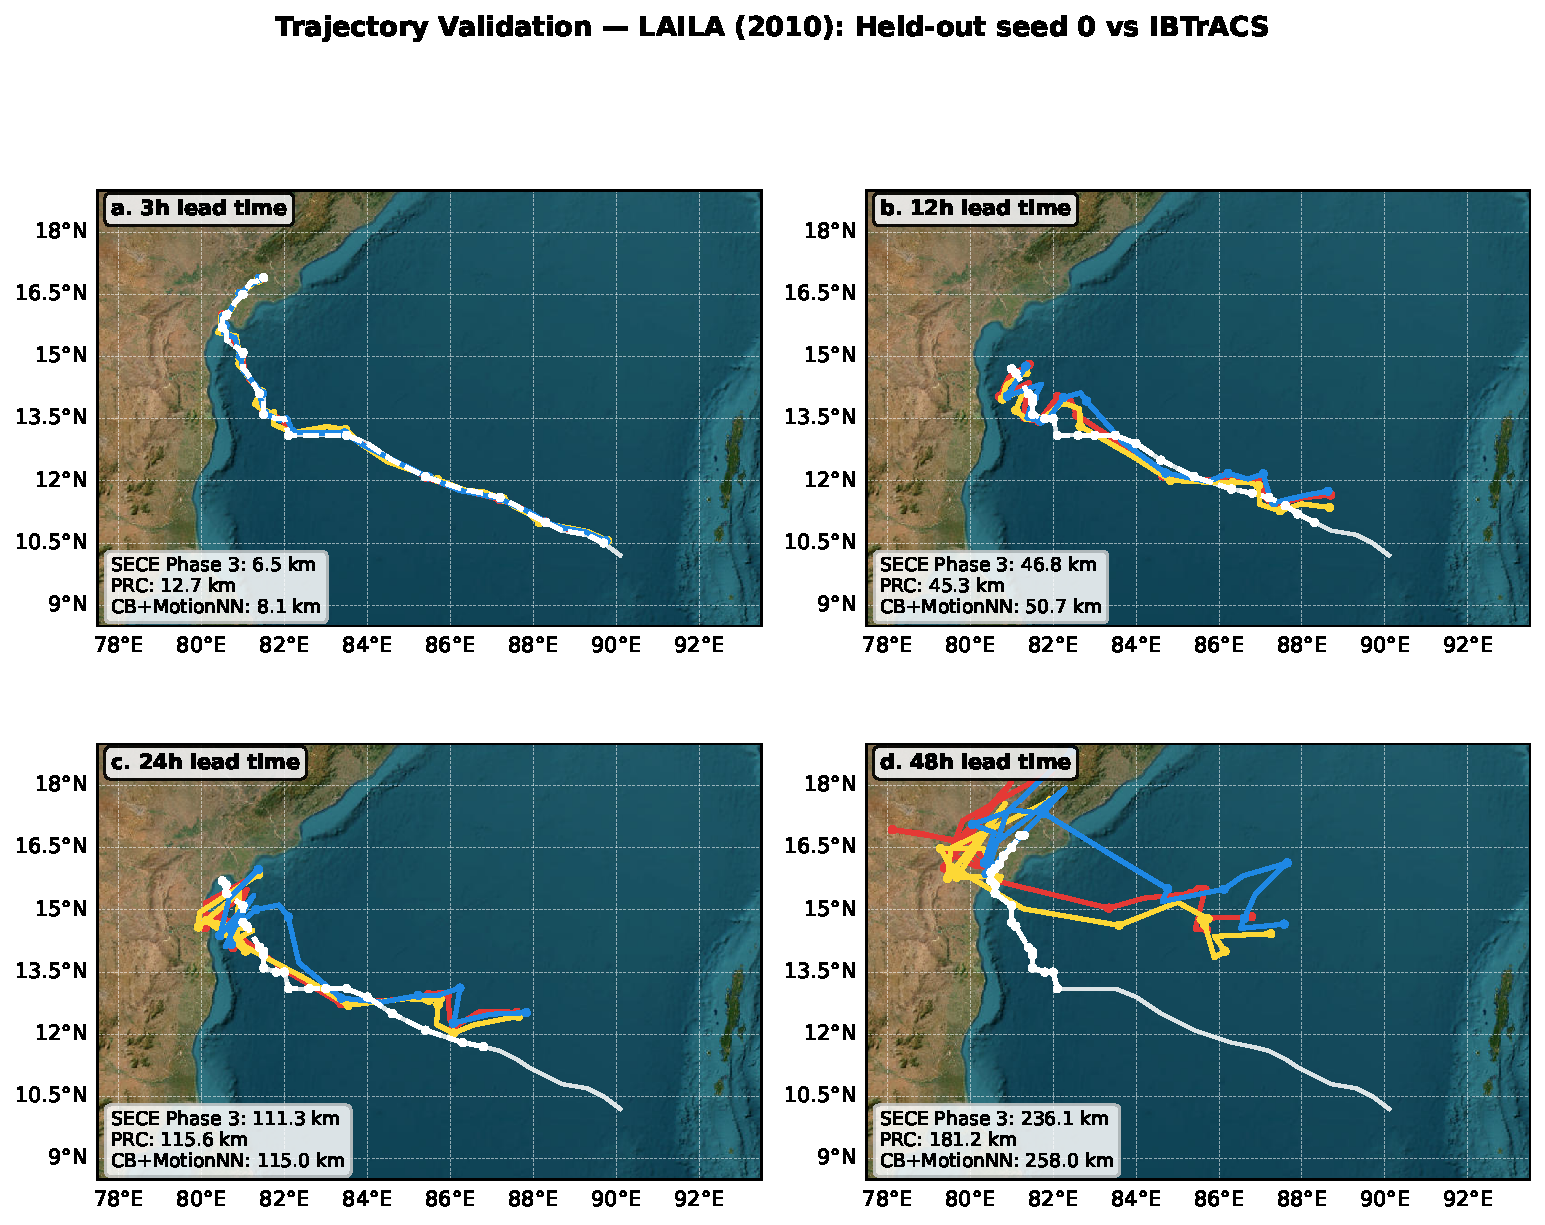
\includegraphics[width=0.98\textwidth]{fig07laila.pdf}
\caption{Cyclone Laila (2010) on held-out seed~0
(\texttt{05\_case\_study\_trajectories.csv}). Four panels: 3, 12, 24, and 48\,h
lead times. White solid line: storm centre at each forecast origin; white dashed
with markers: verified \ibtracs{} position at that lead. Red, yellow, and blue
tracks are \sece{} Phase~3, PRC, and CB+MotionNN endpoints from each origin (not a
recursively rolled-out trajectory). Panel legends give median great-circle error
(km) for those three systems on this storm.}
\label{fig:laila}
\end{figure}

Fig.~\ref{fig:laila} shows predicted and observed tracks for a held-out storm.
Each marker is a prediction issued from a distinct origin time along the
trajectory and offset forward by the panel's lead time, so the panels show direct
multi-horizon endpoints rather than a recursively rolled-out track. Where a
competitor is drawn, it is the system with the lowest \emph{pooled} held-out median
at that horizon, namely Random Forest at 3\,h, stacking at 12 and 24\,h, and
XGBoost at 48\,h, which is not necessarily the best system on the individual storm
shown. The distinction matters in practice, as the following two cases
demonstrate.

\textbf{Cyclone Laila, 2010.} Among the 88 test storms on the diagnostic seed,
Laila exhibits the largest single-storm \era{} benefit for the LightGBM diagnostic
of Section~\ref{sec:diag}: a 25.0\,km improvement at 24\,h and 107.0\,km at 48\,h
when \era{} features are included. We report this as an illustration of that
mechanism, a plain gradient-boosted model's response to atmospheric information,
and not as a claim about \sece{}'s performance on this storm. Separately, at the
ensemble level, \sece{}'s own per-storm error on Laila is 111.3\,km at 24\,h,
locally better than the pooled-best competitor at 128.9\,km, while at 48\,h the
pattern reverses and XGBoost is locally stronger, 204.9 against 236.1\,km,
consistent with the pooled 48\,h leaderboard.

\textbf{A representative 1996 system.} To illustrate typical rather than extreme
behaviour we select the test storm whose \sece{} per-storm median error is closest
to that seed's overall \sece{} 24\,h median of 106.43\,km. This is an unnamed 1996
storm tracking through the central \bob{} with genesis near 8.4$^\circ$N,
87.7$^\circ$E, whose per-storm median error of 107.24\,km closely matches the
typical-case benchmark. On this storm \sece{} at 107.2\,km and the pooled-best
competitor at 110.7\,km are closely matched at 24\,h, while XGBoost shows a wider
local advantage at 48\,h, 276.0 against 306.3\,km. Both cases are consistent with
the aggregate finding that \sece{}'s advantage concentrates at shorter horizons.

% =============================================================================
\section{Discussion}
\label{sec:discussion}
% =============================================================================
The central empirical finding of this study is horizon-dependent. \sece{}'s
context-aware, ensemble-of-experts architecture provides a statistically robust
advantage at short to medium lead times, 3 and 12\,h, where storm-level context
such as recurvature proxies, coastal proximity, and atmospheric steering carries
strong learnable signal. That advantage does not persist as statistically
distinguishable superiority at 24 and 48\,h, where \sece{} instead achieves parity
with, and never significant inferiority to, the strongest available baselines.

We interpret this pattern from a bias-variance perspective on ensemble complexity.
As target uncertainty grows with lead time, the marginal value of additional
ensemble sophistication diminishes, and a comparatively simpler, well-regularised
stacking approach becomes competitive. This extends the finding of \citet{grinsztajn2022tree}, that tree-based methods
outperform deep learning on
tabular data at this scale, by one level: \emph{within} the tree-based ensemble
family, complexity itself should be calibrated to the information content
available at a given forecast horizon rather than applied
uniformly~\citep{ganaie2022ensemble}. The effect sizes in
Table~\ref{tab:wilcox} trace that calibration quantitatively, collapsing from
$-0.208$ against stacking at 3\,h to $-0.071$ at 24\,h.

\era{} features provide genuine value, but the locus of that value differs from
where \sece{}'s architectural advantage is clearest. The per-storm LightGBM
diagnostic of Section~\ref{sec:diag} places \era{}'s majority-of-storms benefit at
48\,h, and the gain shares of Section~\ref{sec:fi} agree, roughly tripling from 24
to 48\,h. The environ-expert architectural addition, by contrast, delivered its
clearest ensemble-level gain at 24\,h. We read this as genuine if imperfectly
aligned confirmation that atmospheric information and ensemble architecture
contribute complementary rather than identical improvements, and we flag the
alignment between them as a direction for further investigation rather than a
discrepancy to be smoothed over.

For operational interpretation, the horizons at which \sece{} is significantly
better are also the horizons that govern short-fuse decisions such as port
closure and shelter activation, whereas 24 to 48\,h guidance is better treated as
a consensus problem in which several strong systems are statistically
interchangeable~\citep{goerss2000tropical,goerss2004tropical}. A practitioner
choosing a single system for this basin could reasonably run \sece{} for
short-range guidance and a simpler stack or persistence-residual model at long
range, and our tables give the evidence for that split rather than a blanket
recommendation.

Operational context clarifies what those medians do and do not imply. RSMC New
Delhi verifies official tropical-cyclone track forecasts over the North Indian
Ocean using WMO-standard direct position error against IMD best
track~\citep{mohapatra2013imdtrack}. For verified forecasts in 2009--2013,
published mean errors were 124.1\,km at 24\,h and 202.1\,km at
48\,h~\citep{mohapatra2013imdtrack}. Our held-out \sece{} pooled medians are
101.2 and 246.3\,km at the same leads. Those figures are \emph{not} directly
comparable: we score retrospective IBTrACS origins with a fixed ML hindcast, whereas
IMD errors average operational issuances from deep depression onward on a
year-specific storm sample. We therefore do not claim to beat the operational
multi-model ensemble or dynamical--statistical Cyclone Prediction System; this
confirm benchmarks learned systems against each other. The comparison shows only
that 24\,h ML errors sit in the same order of magnitude as published official
24\,h verification, while 48\,h ML medians remain broadly consistent with the
difficulty of extended-range track guidance in this basin.

Finally, the leakage correction of Section~\ref{sec:leakage} is not an ancillary
methodological remark but the reason the preceding claims are credible. Our
pre-correction architecture appeared to win at every horizon, and that apparent
sweep did not replicate on fresh seeds. The agreement between the development and
held-out tiers after freezing, 246.94 against 246.99\,km at 48\,h, is the evidence
that the locked design generalises, and it is evidence of a kind that only a
firewalled confirm can produce~\citep{cawley2010}.

% =============================================================================

\FloatBarrier
\section{Limitations}
\label{sec:limits}

\textbf{Environmental fields.} The locked model uses \era{} only at the storm
centre (14 point variables). We tested 5$^\circ$ and 3$^\circ$ spatial-patch
statistics in development; they did not improve 24--48\,h mean error enough to
justify adoption (Table~\ref{tab:abl}; Fig.~\ref{fig:ablation}), remaining
inside seed noise relative to the environ expert. Gridded or attention-based
encoders therefore remain outside this benchmark.

\textbf{Deterministic outputs.} Every system returns a single track point
without forecast spread. That omission matters most at 24--48\,h, where
Table~\ref{tab:heldout} shows overlapping leading medians and right-skewed
errors. A probabilistic formulation trained under a proper scoring
rule~\citep{gneiting2007} is future work, not a result claimed here.

\textbf{Baseline scope.} The confirm table is an eight-way tree and hybrid
comparison. CNN-GRU and BLSTM were not re-trained on the locked \era{} protocol;
section~\ref{sec:dlscope} summarises exploratory development under the uniform
budget~\citep{grinsztajn2022tree}. Tuned deep encoders on gridded \era{} remain
future work.

\textbf{Historical mixing.} Genesis 1940--2024 spans pre-satellite and modern
eras. A fixed modern holdout (section~\ref{sec:window}) supports the wide window
for track error, yet pre-1979 wind-observation sparsity limits
intensity-adjacent interpretation, and residual confounding between sample size
and observational era cannot be fully excluded.

\textbf{Basin scope and transfer.} Feature subsets, router menus, and confirm
statistics are tuned to North Indian Ocean genesis and \bob{} steering regimes
(monsoon trough interaction, shallow funnel geometry, land proximity). We report
no zero-shot or retrained evaluation on the Western North Pacific, Atlantic, or
other basins; cross-basin transfer remains strictly future work.

\textbf{Attribution.} Section~\ref{sec:fi} and Fig.~\ref{fig:featimp} report
LightGBM \emph{gain} on the environ expert for held-out seed~0 only. This is
illustrative, not multi-seed SHAP or permutation testing, and not mechanistic
proof of how atmospheric fields cause track-error reductions.

\section{Conclusion}
\label{sec:conclusion}
% =============================================================================
We present a leakage-corrected, statistically validated, \era{}-augmented
benchmark for multi-horizon tropical cyclone track prediction over the \bob{}. The
proposed ensemble, \sece{} v2 Phase~3, significantly outperforms seven baseline
systems at 3 and 12\,h lead times and achieves statistical parity with the
strongest baselines at 24 and 48\,h, never falling to significant inferiority at
any tested horizon among the evaluated tree-based systems. We identify and correct
a test-set leakage failure mode encountered during our own development, document a
controlled ablation isolating the contribution of \era{} atmospheric features, and
report negative results, specifically the rejection of spatial-patch features,
alongside the positive ones. The intent is a complete and reproducible account of
what this class of model can and cannot currently achieve for an operationally
important and underserved region.

% =============================================================================

\acknowledgments
ERA5 reanalysis fields were obtained from the Copernicus Climate Data Store
\citep{hersbach2023era5}. IBTrACS best-track data were obtained from NOAA's
National Centers for Environmental Information \citep{knapp2010ibtracs,gahtan2024ibtracs}.
The authors declare no conflicts of interest.

\datastatement
Processed modelling tables, locked held-out predictions, bootstrap and Wilcoxon
outputs, case-study trajectories, seed lists, and split counts are versioned with
the project. ERA5 is available from the Copernicus Climate Data Store
(https://doi.org/10.24381/cds.adbb2d47). IBTrACS version 4r01 is available from
NOAA NCEI (https://doi.org/10.25921/82ty-9e16). Every new figure in this
manuscript regenerates from those frozen files.

% REFERENCES -- copied verbatim from the reviewed submission source.
% Do not add entries from memory. Unresolved NEEDS-VERIFICATION-* keys are
% intentional and listed in CITATION_PLACEHOLDERS.md.
% =============================================================================
\begin{thebibliography}{40}

\bibitem[Knapp et al.(2010)]{knapp2010ibtracs}
K. R. Knapp, M. C. Kruk, D. H. Levinson, H. J. Diamond, and C. J. Neumann, ``The International Best Track Archive for Climate Stewardship (IBTrACS): Unifying tropical cyclone best track data,'' \textit{Bulletin of the American Meteorological Society}, vol. 91, no. 3, pp. 363--376, Mar. 2010.

\bibitem[Gahtan et al.(2024)]{gahtan2024ibtracs}
J. Gahtan, K. R. Knapp, C. J. Schreck, H. J. Diamond, and J. P. Kossin, ``International Best Track Archive for Climate Stewardship (IBTrACS) Project, Version 4r01,'' NOAA National Centers for Environmental Information, 2024. [Online]. Available: https://doi.org/10.25921/82ty-9e16

\bibitem[World Bank(2007)]{worldbank2007sidr}
World Bank, ``Cyclone Sidr in Bangladesh: Damage, Loss, and Needs Assessment for Disaster Recovery and Reconstruction,'' Washington, DC, USA, Tech. Rep., 2007.

\bibitem[Paul(2013)]{paul2013post}
S. Paul, ``Post-cyclone livelihood status and strategies in coastal Bangladesh,'' \textit{Rajshahi University Journal of Life \& Earth and Agricultural Sciences}, vol. 41, pp. 1--20, 2013.

\bibitem[IFRC(2020)]{ifrc2020amphan}
International Federation of Red Cross and Red Crescent Societies, ``Emergency Plan of Action (EPoA) Bangladesh: Cyclone Amphan,'' Geneva, Switzerland, Tech. Rep., May 2020.

\bibitem[World Bank(2023)]{worldbank2023mocha}
World Bank, ``Global Rapid Post-Disaster Damage Estimation (GRADE) Report: Extremely Severe Tropical Cyclone Mocha, May 2023 -- Myanmar,'' Washington, DC, USA, Tech. Rep., 2023.

% \bibitem[Gomez et al.(2026)]{gomez2026tcbench}
% M. Gomez et al., ``TCBench: A Benchmark for Tropical Cyclone Track and Intensity Forecasting at the Global Scale,'' \textit{arXiv preprint arXiv:2601.23268}, 2026.

\bibitem[Gomez et al.(2026)]{gomez2026tcbench}
M. Gomez, M. McGraw, S. Ganesh, F. I.-H. Tam, I. Azizi, S. Darmon, M. Feldmann, S. Bourdin, L. Poulain--Auz\'{e}au, S. J. Camargo, J. Lin, D. Chavas, C.-Y. Lee, R. Gupta, A. Jenney, and T. Beucler, ``TCBench: A Benchmark for Tropical Cyclone Track and Intensity Forecasting at the Global Scale,'' \textit{arXiv preprint arXiv:2601.23268}, 2026. [Online]. Available: \url{https://arxiv.org/abs/2601.23268}

\bibitem[Lian et al.(2020)]{lian2020novel}
J. Lian, P. Dong, Y. Zhang, J. Pan, and K. Liu, ``A novel data-driven tropical cyclone track prediction model based on CNN and GRU with multi-dimensional feature selection,'' \textit{IEEE Access}, vol. 8, pp. 97114--97128, 2020. doi: 10.1109/ACCESS.2020.2992083.

\bibitem[Alemany et al.(2019)]{alemany2019predicting}
S. Alemany, J. Beltran, A. Perez, and S. Ganzfried, ``Predicting hurricane trajectories using a recurrent neural network,'' in \textit{Proc. AAAI Conf. Artificial Intelligence}, vol. 33, Honolulu, Hawaii, USA, 2019, pp. 468--475.

\bibitem[Giffard-Roisin et al.(2020)]{giffard2020tropical}
S. Giffard-Roisin, M. Yang, G. Charpiat, C. K. Bonfanti, B. K\'{e}gl, and C. Monteleoni, ``Tropical cyclone track forecasting using fused deep learning from aligned reanalysis data,'' \textit{Frontiers in Big Data}, vol. 3, p. 1, Jan. 2020.

\bibitem[Kar and Banerjee(2021)]{kar2021tropical}
C. Kar and S. Banerjee, ``Tropical cyclone intensity prediction using best track data over North Indian Ocean by machine learning classifiers,'' in \textit{2021 IEEE International India Geoscience and Remote Sensing Symposium (InGARSS)}, pp. 297--300, Dec. 2021.

\bibitem[Goerss(2004)]{goerss2004tropical}
J. S. Goerss, ``Tropical Cyclone Track Forecasts Using an Ensemble of Dynamical Models,'' \textit{Weather and Forecasting}, vol. 19, no. 2, pp. 255--263, Apr. 2004.

\bibitem[Ganaie et al.(2022)]{ganaie2022ensemble}
M. A. Ganaie, M. Hu, A. K. Malik, M. Tanveer, and P. N. Suganthan, ``Ensemble deep learning: A review,'' \textit{Engineering Applications of Artificial Intelligence}, vol. 115, p. 105151, Nov. 2022.

\bibitem[Grinsztajn et al.(2022)]{grinsztajn2022tree}
L. Grinsztajn, E. Oyallon, and G. Varoquaux, ``Why do tree-based models still outperform deep learning on tabular data?,'' in \textit{Proc. 36th Int. Conf. Neural Inf. Process. Syst. (NeurIPS)}, 2022, pp. 507--520.

\bibitem[Neumann(1972)]{neumann1972alternative}
C. J. Neumann, ``An alternate to the HURRAN (Hurricane Analog) Tropical Cyclone Forecast System,'' \textit{NOAA Technical Memorandum}, NWS SR-62, 1972.

\bibitem[Dube et al.(2009)]{dube2009storm}
S. K. Dube, I. Jain, A. D. Rao, and T. S. Murty, ``Storm surge modelling for the Bay of Bengal and Arabian Sea,'' \textit{Natural Hazards}, vol. 51, pp. 3--27, Oct. 2009, doi: 10.1007/s11069-009-9397-9.

\bibitem[Mohapatra et al.(2013)]{mohapatra2013imdtrack}
M. Mohapatra, D. P. Nayak, R. Sharma, and B. K. Bandyopadhyay, ``Evaluation of official tropical cyclone track forecast over north Indian Ocean issued by India Meteorological Department,'' \textit{J. Earth Syst. Sci.}, vol. 122, no. 3, pp. 589--601, 2013, doi: 10.1007/s12040-013-0291-1.

\bibitem[Aberson(1998)]{aberson1998five}
S. D. Aberson, ``Five-day tropical cyclone track forecasts in the North Atlantic basin,'' \textit{Weather and Forecasting}, vol. 13, no. 4, pp. 1005--1015, Dec. 1998.

\bibitem[Goerss(2000)]{goerss2000tropical}
J. S. Goerss, ``Tropical cyclone track forecasts using an ensemble of dynamical models,'' \textit{Monthly Weather Review}, vol. 128, no. 4, pp. 1187--1193, Apr. 2000.

\bibitem[Hossain et al.(2021)]{hossain2021track}
M. S. Hossain, M. A. Samad, M. R. Sultana, M. Mallik, and M. J. Uddin, ``Track and Landfall Characteristics of Very Severe Cyclonic Storm Fani over the Bay of Bengal using WRF Model,'' \textit{Dhaka University Journal of Science}, vol. 69, no. 2, pp. 101--108, Dec. 2021.

\bibitem[Rahman et al.(2025)]{rahman2025tropical}
S. Rahman, M. F. Faisal, P. Mondal, and M. M. Rahman, ``Tropical cyclone track prediction harnessing deep learning algorithms: A comparative study on the Northern Indian Ocean,'' \textit{Results in Engineering}, vol. 26, Art.\ no.\ 105009, 2025, doi: 10.1016/j.rineng.2025.105009. [Online]. Available: \url{https://www.sciencedirect.com/science/article/pii/S2590123025010849}

\bibitem[Kumar et al.(2024)]{kumar2024machine}
S. Kumar, A. K. Singh, and R. K. Jaiswal, ``Machine learning-based tropical cyclone track and intensity prediction: A comprehensive review,'' \textit{Natural Hazards Review}, vol. 25, no. 2, p. 03124001, 2024.

\bibitem[Qu et al.(2025)]{qu2025accurate}
H. Qu, H. Xu, L. Dong, C. Xiang, and G. Nie, ``Accurate typhoon intensity forecasts using a non-iterative spatiotemporal transformer model,'' arXiv preprint arXiv:2509.21349, Sep. 2025.

\bibitem[Chen and Guestrin(2016)]{chen2016xgboost}
T. Chen and C. Guestrin, ``XGBoost: A scalable tree boosting system,'' in \textit{Proc. 22nd ACM SIGKDD Int. Conf. Knowledge Discovery and Data Mining}, San Francisco, CA, USA, 2016, pp. 785--794.

\bibitem[Ke et al.(2017)]{ke2017lightgbm}
G. Ke, Q. Meng, T. Finley, T. Wang, W. Chen, W. Ma, Q. Ye, and T. Y. Liu, ``LightGBM: A Highly Efficient Gradient Boosting Decision Tree,'' in \textit{Proc. 31st Int. Conf. Neural Inf. Process. Syst. (NIPS)}, 2017, pp. 3149--3157.

\bibitem[Prokhorenkova et al.(2018)]{prokhorenkova2018catboost}
L. Prokhorenkova, G. Gusev, A. Vorobev, A. V. Dorogush, and A. Gulin, ``CatBoost: unbiased boosting with categorical features,'' in \textit{Proc. 32nd Int. Conf. Neural Inf. Process. Syst. (NeurIPS)}, 2018, pp. 6638--6648.

\bibitem[Hersbach et al.(2023)]{hersbach2023era5}
H. Hersbach et al., ``ERA5 hourly data on single levels from 1940 to present,'' Copernicus Climate Change Service (C3S) Climate Data Store (CDS), 2023. [Online]. Available: https://doi.org/10.24381/cds.adbb2d47

\bibitem[Krishnamurti et al.(2010)]{krishnamurti2010ann}
T. N. Krishnamurti, A. K. Mishra, A. Simon, A. Semazzi, and H. S. Bhardwaj, ``Predicting cyclone tracks in the north Indian Ocean: An artificial neural network approach,'' \textit{Geophys. Res. Lett.}, vol. 37, no. 20, L19801, 2010, doi: 10.1029/2010GL044718.

\bibitem[Pan(2024)]{pan2024guangdong}
C. Pan, ``A Study on The Frequency Characteristics of Typhoon Landing in Guangdong, China, Based on Machine Learning Methods,'' in \textit{Proc. ISCRAM 2024}, 2024, doi: 10.59297/zb59g660.

\bibitem[Breiman(2001)]{breiman2001rf}
L. Breiman, ``Random forests,'' \textit{Machine Learning}, vol. 45, no. 1, pp. 5--32, Oct. 2001, doi: 10.1023/A:1010933404324.

\bibitem[van der Maaten and Hinton(2008)]{maaten2008tsne}
L. van der Maaten and G. Hinton, ``Visualizing data using t-SNE,'' \textit{Journal of Machine Learning Research}, vol. 9, pp. 2579--2605, 2008.

\bibitem[Hochreiter and Schmidhuber(1997)]{hochreiter1997lstm}
S. Hochreiter and J. Schmidhuber, ``Long short-term memory,'' \textit{Neural Computation}, vol. 9, no. 8, pp. 1735--1780, Nov. 1997.

\bibitem[Cho et al.(2014)]{cho2014gru}
K. Cho, B. van Merrienboer, C. Gulcehre, D. Bahdanau, F. Bougares, H. Schwenk, and Y. Bengio, ``Learning phrase representations using RNN encoder-decoder for statistical machine translation,'' in \textit{Proc. Conf. Empirical Methods in Natural Language Processing (EMNLP)}, Doha, Qatar, 2014, pp. 1724--1734.

\bibitem[Graves and Schmidhuber(2005)]{graves2005blstm}
A. Graves and J. Schmidhuber, ``Framewise phoneme classification with bidirectional LSTM networks,'' in \textit{Proc. Int. Joint Conf. Neural Networks (IJCNN)}, Montreal, QC, Canada, 2005, pp. 2047--2052.

\bibitem[Vaswani et al.(2017)]{vaswani2017attention}
A. Vaswani, N. Shazeer, N. Parmar, J. Uszkoreit, L. Jones, A. N. Gomez, \L. Kaiser, and I. Polosukhin, ``Attention is all you need,'' in \textit{Advances in Neural Information Processing Systems}, vol. 30, Long Beach, CA, USA, 2017.

\bibitem[Cawley and Talbot(2010)]{cawley2010}
G. C. Cawley and N. L. C. Talbot, ``On Over-fitting in Model Selection and Subsequent Selection Bias in Performance Evaluation,'' \textit{Journal of Machine Learning Research}, vol. 11, no. 70, pp. 2079--2107, 2010.

\bibitem[Efron(1979)]{efron1979}
B. Efron, ``Bootstrap Methods: Another Look at the Jackknife,'' \textit{The Annals of Statistics}, vol. 7, no. 1, pp. 1--26, 1979.

\bibitem[Wilcoxon(1945)]{wilcoxon1945}
F. Wilcoxon, ``Individual Comparisons by Ranking Methods,'' \textit{Biometrics Bulletin}, vol. 1, no. 6, pp. 80--83, Dec. 1945.

\bibitem[Bonferroni(1936)]{bonferroni1936}
C. E. Bonferroni, ``Teoria statistica delle classi e calcolo delle probabilit\`a,'' \textit{Pubblicazioni del R Istituto Superiore di Scienze Economiche e Commerciali di Firenze}, vol. 8, pp. 3--62, 1936.

\bibitem[Sinnott(1984)]{sinnott1984}
R. W. Sinnott, ``Virtues of the Haversine,'' \textit{Sky and Telescope}, vol. 68, no. 2, p. 159, 1984.

\bibitem[Gneiting and Raftery(2007)]{gneiting2007}
T. Gneiting and A. E. Raftery, ``Strictly Proper Scoring Rules, Prediction, and Estimation,'' \textit{Journal of the American Statistical Association}, vol. 102, no. 477, pp. 359--378, 2007.

\end{thebibliography}

\end{document}
